% 若编译失败,且生成 .synctex(busy) 辅助文件,可能有两个原因:
% 1. 需要插入的图片不存在:Ctrl + F 搜索 'figure' 将这些代码注释/删除掉即可
% 2. 路径/文件名含中文或空格:更改路径/文件名即可

% --------------------- 文章宏包及相关设置 --------------------- %
% >> ------------------ 文章宏包及相关设置 ------------------ << %
% 设定文章类型与编码格式
\documentclass[UTF8]{article}		

% 物理实验报告所需的其它宏包
\usepackage{ulem}   % \uline 下划线支持
\usepackage{circuitikz} % 电路图 tikz 支持
\usepackage{pdfpages}   % 用于导入 pdf 文件

% 本 .tex 专属的宏定义
    \def\V{\ \mathrm{V}}
    \def\uV{\ \mu\mathrm{V}}
    \def\mV{\ \mathrm{mV}}
    \def\K{\ \mathrm{K}}
    \def\kV{\ \mathrm{KV}}
    \def\KV{\ \mathrm{KV}}
    \def\MV{\ \mathrm{MV}}
    \def\uA{\ \mu\mathrm{A}}
    \def\mA{\ \mathrm{mA}}
    \def\A{\ \mathrm{A}}
    \def\kA{\ \mathrm{KA}}
    \def\KA{\ \mathrm{KA}}
    \def\MA{\ \mathrm{MA}}
    \def\O{\ \Omega}
    \def\mO{\ \Omega}
    \def\kO{\ \mathrm{K}\Omega}
    \def\KO{\ \mathrm{K}\Omega}
    \def\MO{\ \mathrm{M}\Omega}
    \def\Hz{\ \mathrm{Hz}}
    \def\uF{\ \mu\mathrm{F}}
    \def\mF{\ \mathrm{mF}}
    \def\F{\ \mathrm{F}}
    \def\Re{\mathrm{\,Re}\,}
    \def\Im{\mathrm{\,Im}\,}
    \def\sinc{\mathrm{\,sinc}\,}

% 自定义宏定义
    \def\N{\mathbb{N}}
    \def\F{\mathbb{F}}
    \def\Z{\mathbb{Z}}
    \def\Q{\mathbb{Q}}
    \def\R{\mathbb{R}}
    \def\C{\mathbb{C}}
    \def\T{\mathbb{T}}
    \def\S{\mathbb{S}}
    %\def\A{\mathbb{A}}
    \def\I{\mathscr{I}}
    \def\d{\mathrm{d}}
    \def\p{\partial}


% 导入基本宏包
    \usepackage[UTF8]{ctex}     % 设置文档为中文语言
    \usepackage{hyperref}  % 宏包:自动生成超链接 (此宏包与标题中的数学环境冲突)
    \hypersetup{
        colorlinks=true,    % false:边框链接 ; true:彩色链接
        citecolor={blue},    % 文献引用颜色
        linkcolor={blue},   % 目录 (我们在目录处单独设置),公式,图表,脚注等内部链接颜色
        urlcolor={magenta},    % 网页 URL 链接颜色,包括 \href 中的 text
        % cyan 浅蓝色 
        % magenta 洋红色
        % yellow 黄色
        % black 黑色
        % white 白色
        % red 红色
        % green 绿色
        % blue 蓝色
        % gray 灰色
        % darkgray 深灰色
        % lightgray 浅灰色
        % brown 棕色
        % lime 石灰色
        % olive 橄榄色
        % orange 橙色
        % pink 粉红色
        % purple 紫色
        % teal 蓝绿色
        % violet 紫罗兰色
    }
    % \usepackage{docmute}    % 宏包:子文件导入时自动去除导言区,用于主/子文件的写作方式,\include{./51单片机笔记}即可。注:启用此宏包会导致.tex文件capacity受限。
    \usepackage{amsmath}    % 宏包:数学公式
    \usepackage{mathrsfs}   % 宏包:提供更多数学符号
    \usepackage{amssymb}    % 宏包:提供更多数学符号
    \usepackage{pifont}     % 宏包:提供了特殊符号和字体
    \usepackage{extarrows}  % 宏包:更多箭头符号 
    \usepackage{multicol}   % 宏包:支持多栏 

% 文章页面margin设置
    \usepackage[a4paper]{geometry}
        \geometry{top=0.75in}
        \geometry{bottom=0.75in}
        \geometry{left=0.75in}
        \geometry{right=0.75in}   % 设置上下左右页边距
        \geometry{marginparwidth=1.75cm}    % 设置边注距离(注释、标记等)

% 配置数学环境
    \usepackage{amsthm} % 宏包:数学环境配置
    % theorem-line 环境自定义
        \newtheoremstyle{MyLineTheoremStyle}% <name>
            {11pt}% <space above>
            {11pt}% <space below>
            {\kaishu}% <body font> 默认使用正文字体, \kaishu 为楷体
            {}% <indent amount>
            {\bfseries}% <theorem head font> 设置标题项为加粗
            {:\ \ }% <punctuation after theorem head>
            {.5em}% <space after theorem head>
            {\textbf{#1}\thmnumber{#2}\ \ (\,\textbf{#3}\,)}% 设置标题内容顺序
        \theoremstyle{MyLineTheoremStyle} % 应用自定义的定理样式
        \newtheorem{LineTheorem}{Theorem.\,}
    % theorem-block 环境自定义
        \newtheoremstyle{MyBlockTheoremStyle}% <name>
            {11pt}% <space above>
            {11pt}% <space below>
            {\kaishu}% <body font> 使用默认正文字体
            {}% <indent amount>
            {\bfseries}% <theorem head font> 设置标题项为加粗
            {:\\ \indent}% <punctuation after theorem head>
            {.5em}% <space after theorem head>
            {\textbf{#1}\thmnumber{#2}\ \ (\,\textbf{#3}\,)}% 设置标题内容顺序
        \theoremstyle{MyBlockTheoremStyle} % 应用自定义的定理样式
        \newtheorem{BlockTheorem}[LineTheorem]{Theorem.\,} % 使用 LineTheorem 的计数器
    % definition 环境自定义
        \newtheoremstyle{MySubsubsectionStyle}% <name>
            {11pt}% <space above>
            {11pt}% <space below>
            {}% <body font> 使用默认正文字体
            {}% <indent amount>
            {\bfseries}% <theorem head font> 设置标题项为加粗
            {:\\ \indent}% <punctuation after theorem head>
            {0pt}% <space after theorem head>
            {\textbf{#3}}% 设置标题内容顺序
        \theoremstyle{MySubsubsectionStyle} % 应用自定义的定理样式
        \newtheorem{definition}{}

%宏包:有色文本框(proof环境)及其设置
\usepackage{xcolor}    %设置插入的文本框颜色
    % rgb(4, 9, 103), rgb(5, 13, 164)
    % rgb(124, 131, 255), rgb(231, 232, 255)
    % rgb(255, 190, 190), rgb(255, 70, 70)
    \definecolor{stc}{RGB}{4, 10, 118}  % 设置各级标题结构颜色
\usepackage[strict]{changepage}     % 提供一个 adjustwidth 环境
\usepackage{framed}     % 实现方框效果
    % rgb(0, 0, 0), rgb(100, 100, 100)
    %#ECECED 为 0.93, 0.93, 0.93
    \definecolor{graybox_color}{rgb}{0.93, 0.93, 0.93} % 这里的 rbg 范围是 [0, 1]
    % 文本框颜色。修改此行中的 rgb 数值即可改变方框纹颜色,具体颜色的rgb数值可以在网站https://colordrop.io/ 中获得。(截止目前的尝试还没有成功过,感觉单位不一样)(找到喜欢的颜色,点击下方的小眼睛,找到rgb值,复制修改即可)
    \newenvironment{graybox}{%
    \def\FrameCommand{%
    \hspace{1pt}%
    {\color{gray}\small \vrule width 2pt}%
    {\color{graybox_color}\vrule width 4pt}%
    \colorbox{graybox_color}%
    }%
    \MakeFramed{\advance\hsize-\width\FrameRestore}%
    \noindent\hspace{-4.55pt}% disable indenting first paragraph
    \begin{adjustwidth}{}{7pt}%
    \vspace{2pt}\vspace{2pt}%
    }
    {%
    \vspace{2pt}\end{adjustwidth}\endMakeFramed%
    }

    \definecolor{bluebox_ruleColor}{rgb}{0.49, 0.51, 1} % 文本框颜色。修改此行中的 rgb 数值即可改变方框纹颜色,具体颜色的rgb数值可以在网站https://colordrop.io/ 中获得。(截止目前的尝试还没有成功过,感觉单位不一样)(找到喜欢的颜色,点击下方的小眼睛,找到rgb值,复制修改即可)
    \definecolor{bluebox_backgroundColor}{rgb}{0.93, 0.93, 1}
    \newenvironment{bluebox}{%
    \def\FrameCommand{%
    \hspace{1pt}%
    {\color{bluebox_ruleColor}\small \vrule width 2pt}%
    {\color{bluebox_backgroundColor}\vrule width 4pt}% 4pt 缩进比较合适
    \colorbox{bluebox_backgroundColor}%
    }%
    \MakeFramed{\advance\hsize-\width\FrameRestore}%
    \noindent\hspace{-4.55pt}% disable indenting first paragraph
    \begin{adjustwidth}{}{7pt}%
    \vspace{2pt}\vspace{2pt}%
    }
    {%
    \vspace{2pt}\end{adjustwidth}\endMakeFramed%
    }

    \definecolor{redbox_ruleColor}{rgb}{1, 0.27, 0.27} % 文本框颜色。修改此行中的 rgb 数值即可改变方框纹颜色,具体颜色的rgb数值可以在网站https://colordrop.io/ 中获得。(截止目前的尝试还没有成功过,感觉单位不一样)(找到喜欢的颜色,点击下方的小眼睛,找到rgb值,复制修改即可)
    \definecolor{redbox_backgroundColor}{rgb}{1, 0.90, 0.90}
    \newenvironment{redbox}{%
    \def\FrameCommand{%
    \hspace{1pt}%
    {\color{redbox_ruleColor}\small \vrule width 2pt}%
    {\color{redbox_backgroundColor}\vrule width 4pt}% 4pt 缩进比较合适
    \colorbox{redbox_backgroundColor}%
    }%
    \MakeFramed{\advance\hsize-\width\FrameRestore}%
    \noindent\hspace{-4.55pt}% disable indenting first paragraph
    \begin{adjustwidth}{}{7pt}%
    \vspace{2pt}\vspace{2pt}%
    }
    {%
    \vspace{2pt}\end{adjustwidth}\endMakeFramed%
    }

% 外源代码插入设置
    % matlab 代码插入设置
    \usepackage{matlab-prettifier}
        \lstset{style=Matlab-editor}    % 继承 matlab 代码高亮 , 此行不能删去
    \usepackage[most]{tcolorbox} % 引入tcolorbox包 
    \usepackage{listings} % 引入listings包
        \tcbuselibrary{listings, skins, breakable}
        \newfontfamily\codefont{Consolas} % 定义需要的 codefont 字体
        \lstdefinestyle{MatlabStyle_inc}{   % 插入代码的样式
            language=Matlab,
            basicstyle=\footnotesize\ttfamily\codefont,    % ttfamily 确保等宽 
            breakatwhitespace=false,
            breaklines=true,
            captionpos=b,
            keepspaces=true,
            numbers=left,
            numbersep=15pt,
            showspaces=false,
            showstringspaces=false,
            showtabs=false,
            tabsize=2,
            xleftmargin=15pt,   % 左边距
            %frame=single, % single 为包围式单线框
            frame=shadowbox,    % shadowbox 为带阴影包围式单线框效果
            %escapeinside=``,   % 允许在代码块中使用 LaTeX 命令 (此行无用)
            %frameround=tttt,    % tttt 表示四个角都是圆角
            framextopmargin=0pt,    % 边框上边距
            framexbottommargin=0pt, % 边框下边距
            framexleftmargin=5pt,   % 边框左边距
            framexrightmargin=5pt,  % 边框右边距
            rulesepcolor=\color{red!20!green!20!blue!20}, % 阴影框颜色设置
            %backgroundcolor=\color{blue!10}, % 背景颜色
        }
        \lstdefinestyle{MatlabStyle_src}{   % 插入代码的样式
            language=Matlab,
            basicstyle=\small\ttfamily\codefont,    % ttfamily 确保等宽 
            breakatwhitespace=false,
            breaklines=true,
            captionpos=b,
            keepspaces=true,
            numbers=left,
            numbersep=15pt,
            showspaces=false,
            showstringspaces=false,
            showtabs=false,
            tabsize=2,
        }
        \newtcblisting{matlablisting}{
            %arc=2pt,        % 圆角半径
            % 调整代码在 listing 中的位置以和引入文件时的格式相同
            top=0pt,
            bottom=0pt,
            left=-5pt,
            right=-5pt,
            listing only,   % 此句不能删去
            listing style=MatlabStyle_src,
            breakable,
            colback=white,   % 选一个合适的颜色
            colframe=black!0,   % 感叹号后跟不透明度 (为 0 时完全透明)
        }
        \lstset{
            style=MatlabStyle_inc,
        }

% table 支持
    \usepackage{booktabs}   % 宏包:三线表
    \usepackage{tabularray} % 宏包:表格排版
    \usepackage{longtable}  % 宏包:长表格

% figure 设置
    \usepackage{graphicx}  % 支持 jpg, png, eps, pdf 图片 
    \usepackage{svg}       % 支持 svg 图片
        \svgsetup{
            % 指向 inkscape.exe 的路径
            inkscapeexe = C:/aa_MySame/inkscape/bin/inkscape.exe, 
            % 一定程度上修复导入后图片文字溢出几何图形的问题
            inkscapelatex = false                 
        }
    \usepackage{subcaption} % 用于子图和小图注  

% 图表进阶设置
    \usepackage{caption}    % 图注、表注
        \captionsetup[figure]{name=图}  
        \captionsetup[table]{name=表}
        \captionsetup{
            labelfont=bf, % 设置标签为粗体
            textfont=bf,  % 设置文本为粗体
            font=small  
        }
    \usepackage{float}     % 图表位置浮动设置 
    \usepackage{etoolbox} % 用于保证图注表注的数学字符为粗体
        \AtBeginEnvironment{figure}{\boldmath} % 图注中的数学字符为粗体
        \AtBeginEnvironment{table}{\boldmath}  % 表注中的数学字符为粗体
        \AtBeginEnvironment{tabular}{\unboldmath}   % 保证表格中的数学字符不受额外影响

% 圆圈序号自定义
    \newcommand*\circled[1]{\tikz[baseline=(char.base)]{\node[shape=circle,draw,inner sep=0.8pt, line width = 0.03em] (char) {\bfseries #1};}}   % TikZ solution

% 列表设置
    \usepackage{enumitem}   % 宏包:列表环境设置
        \setlist[enumerate]{
            label=(\arabic*) ,   % 设置序号样式为加粗的 (1) (2) (3)
            ref=\arabic*, % 如果需要引用列表项,这将决定引用格式(这里仍然使用数字)
            itemsep=0pt, parsep=0pt, topsep=0pt, partopsep=0pt, leftmargin=3.5em} 
        \setlist[itemize]{itemsep=0pt, parsep=0pt, topsep=0pt, partopsep=0pt, leftmargin=3.5em}
        \newlist{circledenum}{enumerate}{1} % 创建一个新的枚举环境  
        \setlist[circledenum,1]{  
            label=\protect\circled{\arabic*}, % 使用 \arabic* 来获取当前枚举计数器的值,并用 \circled 包装它  
            ref=\arabic*, % 如果需要引用列表项,这将决定引用格式(这里仍然使用数字)
            itemsep=0pt, parsep=0pt, topsep=0pt, partopsep=0pt, leftmargin=3.5em
        }  

% 其它设置
    % 脚注设置
        \renewcommand\thefootnote{\ding{\numexpr171+\value{footnote}}}
    % 参考文献引用设置
        \bibliographystyle{unsrt}   % 设置参考文献引用格式为unsrt
        \newcommand{\upcite}[1]{\textsuperscript{\cite{#1}}}     % 自定义上角标式引用
    % 文章序言设置
        \newcommand{\cnabstractname}{序言}
        \newenvironment{cnabstract}{%
            \par\Large
            \noindent\mbox{}\hfill{\bfseries \cnabstractname}\hfill\mbox{}\par
            \vskip 2.5ex
            }{\par\vskip 2.5ex}

% 文章默认字体设置
    \usepackage{fontspec}   % 宏包:字体设置
        \setmainfont{SimSun}    % 设置中文字体为宋体字体
        \setCJKmainfont[AutoFakeBold=3]{SimSun} % 设置加粗字体为 SimSun 族,AutoFakeBold 可以调整字体粗细
        \setmainfont{Times New Roman} % 设置英文字体为Times New Roman

% 各级标题自定义设置
    \usepackage{titlesec}   
        % section标题自定义设置 
        \titleformat{\section}[hang]{\normalfont\Large\bfseries\boldmath}{\thesection}{8pt}{}
        % subsection 标题自定义设置
        \titleformat{\subsection}[hang]{\normalfont\large\bfseries\boldmath}{\thesubsection}{8pt}{}
        \titlespacing*{\subsection}{0pt}{10pt}{6pt} % 控制上下间距


% --------------------- 文章宏包及相关设置 --------------------- %
% >> ------------------ 文章宏包及相关设置 ------------------ << %




% ------------------------ 文章信息区 ------------------------ %
% ------------------------ 文章信息区 ------------------------ %
% 页眉页脚设置
\usepackage{fancyhdr}   %宏包:页眉页脚设置
    \pagestyle{fancy}
    \fancyhf{}
    \cfoot{\thepage}
    \renewcommand\headrulewidth{1pt}
    \renewcommand\footrulewidth{0pt}
    %\rhead{《线性电路实验》实验报告}    
    \lhead{\small \faGithub\ \href{https://github.com/YiDingg/UCAS-LinearCircuitExperiment}{\color{black} https://github.com/YiDingg/UCAS-LinearCircuitExperiment}}


    \graphicspath{{../}}   % 修改主文件图像路径,使得子文件能够直接使用相对路径,而不是从 assets 开始索引

    \usepackage{fontawesome}    % 宏包:更多符号与图标 (用于插入 GitHub 图标等)



%%%%%%%%%%%%%%%%%%%%%%%%%%%%%%%%%%%%%%%%%%%%%%%%%%%%%%%%%%%%%%%%
% 仅需修改页眉、实验名称、实验日期
%%%%%%%%%%%%%%%%%%%%%%%%%%%%%%%%%%%%%%%%%%%%%%%%%%%%%%%%%%%%%%%%


%%%%%%%%%%%%%%%%%% 1. 修改页眉内容 %%%%%%%%%%%%%%%%%%
\rhead{LCE-05 精密整流 (2025.05.09, 丁毅)}

% 开始编辑文章
\begin{document}
\begin{center}\large
    \vspace*{-0.8cm}
    \noindent{\huge\bfseries《\ \ 线\ \ 性\ \ 电\ \ 路\ \ 实\ \ 验\ \ \ 》\ \ 实\ \ 验\ \ 报\ \ 告 }
    \\\vspace{0.1cm}
    \noindent{
    {\bfseries 
%
%%%%%%%%%%%%%%%%%% 2. 修改实验名称 %%%%%%%%%%%%%%%%%%
    实验名称:\uline{\hspace{2.2cm} xxxxxx \hspace{2.2cm}}
%
    }\hspace{0.4cm}
    指导教师:\uline{\hspace{0.8cm}王东雷\ \ \ \  \ df4dac@sina.com     \hspace{0.8cm}}
    }
    \\\vspace{0.1cm}
    \noindent
    {
    姓名:\uline{\,\,\,丁毅\,\,\,}\hspace{0.2cm}
    学号:\uline{\,\,\,{ 2023K8009908031}\,\,\,}\hspace{0.2cm}
    班级/专业:\uline{\,\,\,{2308/电子信息}\,\,\,}\hspace{0.2cm}
    分组序号:\uline{\,\,\,{2-06}\,\,\,}
    }
    \\\vspace{0.1cm}
    \noindent{
%
%%%%%%%%%%%%%%%%%% 3. 修改实验日期 %%%%%%%%%%%%%%%%%%
    实验日期:\uline{\,\,{2025.05.09}\,\,}\hspace{0.2cm}
%
    实验地点:\uline{\,\,\,教学楼{ 607}\,\,\,}\hspace{0.2cm}
    是否调课/补课:\uline{\hspace{0.26cm}否 \hspace{0.26cm}}\hspace{0.2cm}
    成绩:\uline{\hspace{2cm}}
    }
\end{center}
\vspace{-0.4cm}
\noindent\rule{\textwidth}{0.075em}   % 分割线
\vspace{-1.0cm}

% 生成目录
\setcounter{tocdepth}{3}  % 目录深度为 2(不显示 subsubsection)
\noindent\tableofcontents\thispagestyle{fancy}   % 显示页码、页眉等

% ------------------------ 文章信息区 ------------------------ %
% ------------------------ 文章信息区 ------------------------ %



%%%%%%%%%%%%%%%%%%%%%%%%%%%%%%%%%%%%%%%%%%%%%%%%%%%%%%%%%%%%%%%%%%%%%%%%%%%%%%%%%
%%%%%%%%%%%%%%%%%%%%%%%%%%%%%%%%% 下面是正文内容 %%%%%%%%%%%%%%%%%%%%%%%%%%%%%%%%%
%%%%%%%%%%%%%%%%%%%%%%%%%%%%%%%%%%%%%%%%%%%%%%%%%%%%%%%%%%%%%%%%%%%%%%%%%%%%%%%%%

\section{实验目的}

\begin{enumerate}
    \item 设计由运放构成的精密整流电路,测量波形、精度及带宽;
    \item 加深对有效值定义的理解,了解交流信号检测的方法;
    \item 测试有效值检测电路 AD367,在不同波形下与精密整流电路对比;
    \item 练习使用面包板。
\end{enumerate}
\section{实验仪器}

\begin{enumerate}
    \item 数字万用表: Unit UT61E (C190241394)
    \item 数字示波器: RIGOL 200MSO2202A (DS2F192200361)
    \item 信号发生器: GWINSTEK AFG-22225 (GER910370)
    \item 数字直流电源: GWINSTEK GPD-3303S (GES813705)
    \item 多功能数字测量仪: 
    % 这里是链接
    \href{https://digilent.com/reference/test-and-measurement/analog-discovery/start
    }{ % 这里是文字
    Analog Discovery 1
    } 
    (D704387)
    \item 其它:面包板,运算放大器 LF412,电容、电阻、二极管 (1N4148, 1N5711)、导线等
\end{enumerate}


\section{实验内容及实验结果}

\subsection{TI Absolute Circuit (Diode 1, 1N4148)}
\vspace*{-3mm}
\begin{redbox}
    若无特别说明,后续实验均默认示波器为 dc coupling 模式。
\end{redbox}

\subsubsection{搭建 TI Absolute Circuit (绝对值电路)}

在面包板上搭建 TI Absolute Circuit (绝对值电路),也即我们的精密整流电路,如下图所示:

\begin{figure}[H]\centering
    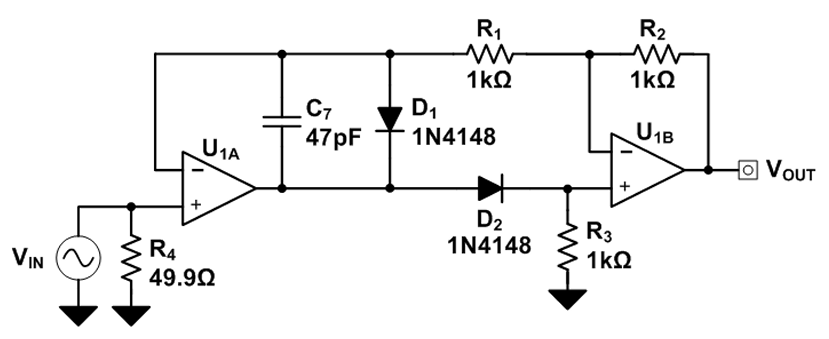
\includegraphics[width=0.7\columnwidth]{LCE-05-精密整流/assets/TI absolute.png}
    \caption{TI verified design: precision full-wave rectifier, dual-supply}
    \label{TI Verified Design: Precision Full-Wave Rectifier, Dual-Supply}
\end{figure}

\begin{figure}[H]\centering
    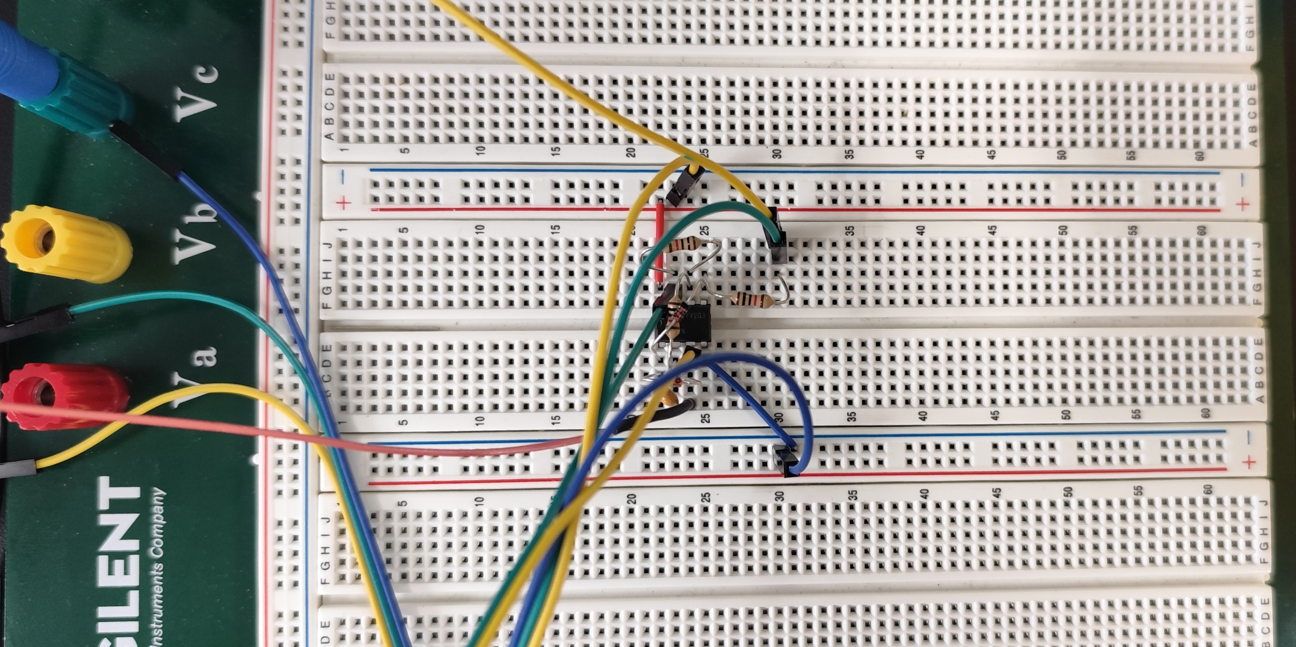
\includegraphics[width=\columnwidth]{LCE-05-精密整流/assets/1N4148/circuit.png}
    \caption{在面包板上搭建 TI precision full-wave rectifier}
\end{figure}

\begin{figure}[H]\centering
    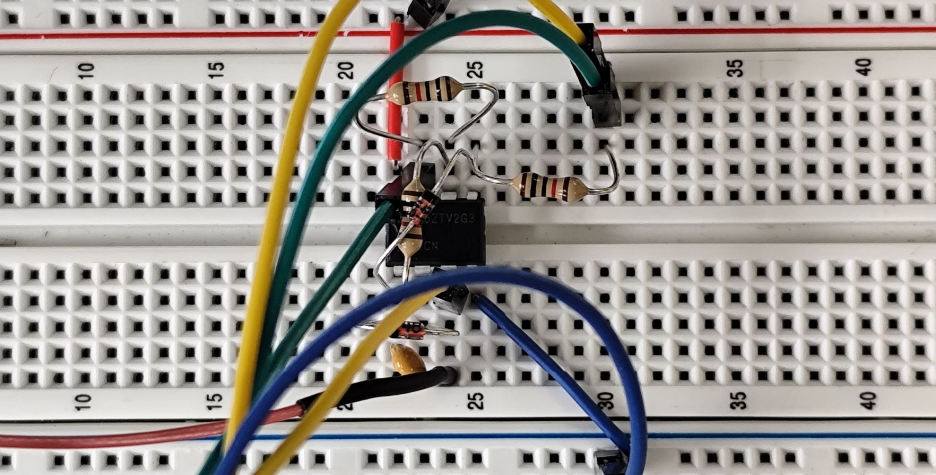
\includegraphics[width=\columnwidth]{LCE-05-精密整流/assets/1N4148/circuit 2.png}
    \caption{在面包板上搭建 TI precision full-wave rectifier (细节展示)}
\end{figure}


\subsubsection{测量低频输入输出波形}

调整输入信号为 sine wave (5 Vamp @ 50 Hz),测量输入输出波形如下:

\begin{figure}[H]\centering
    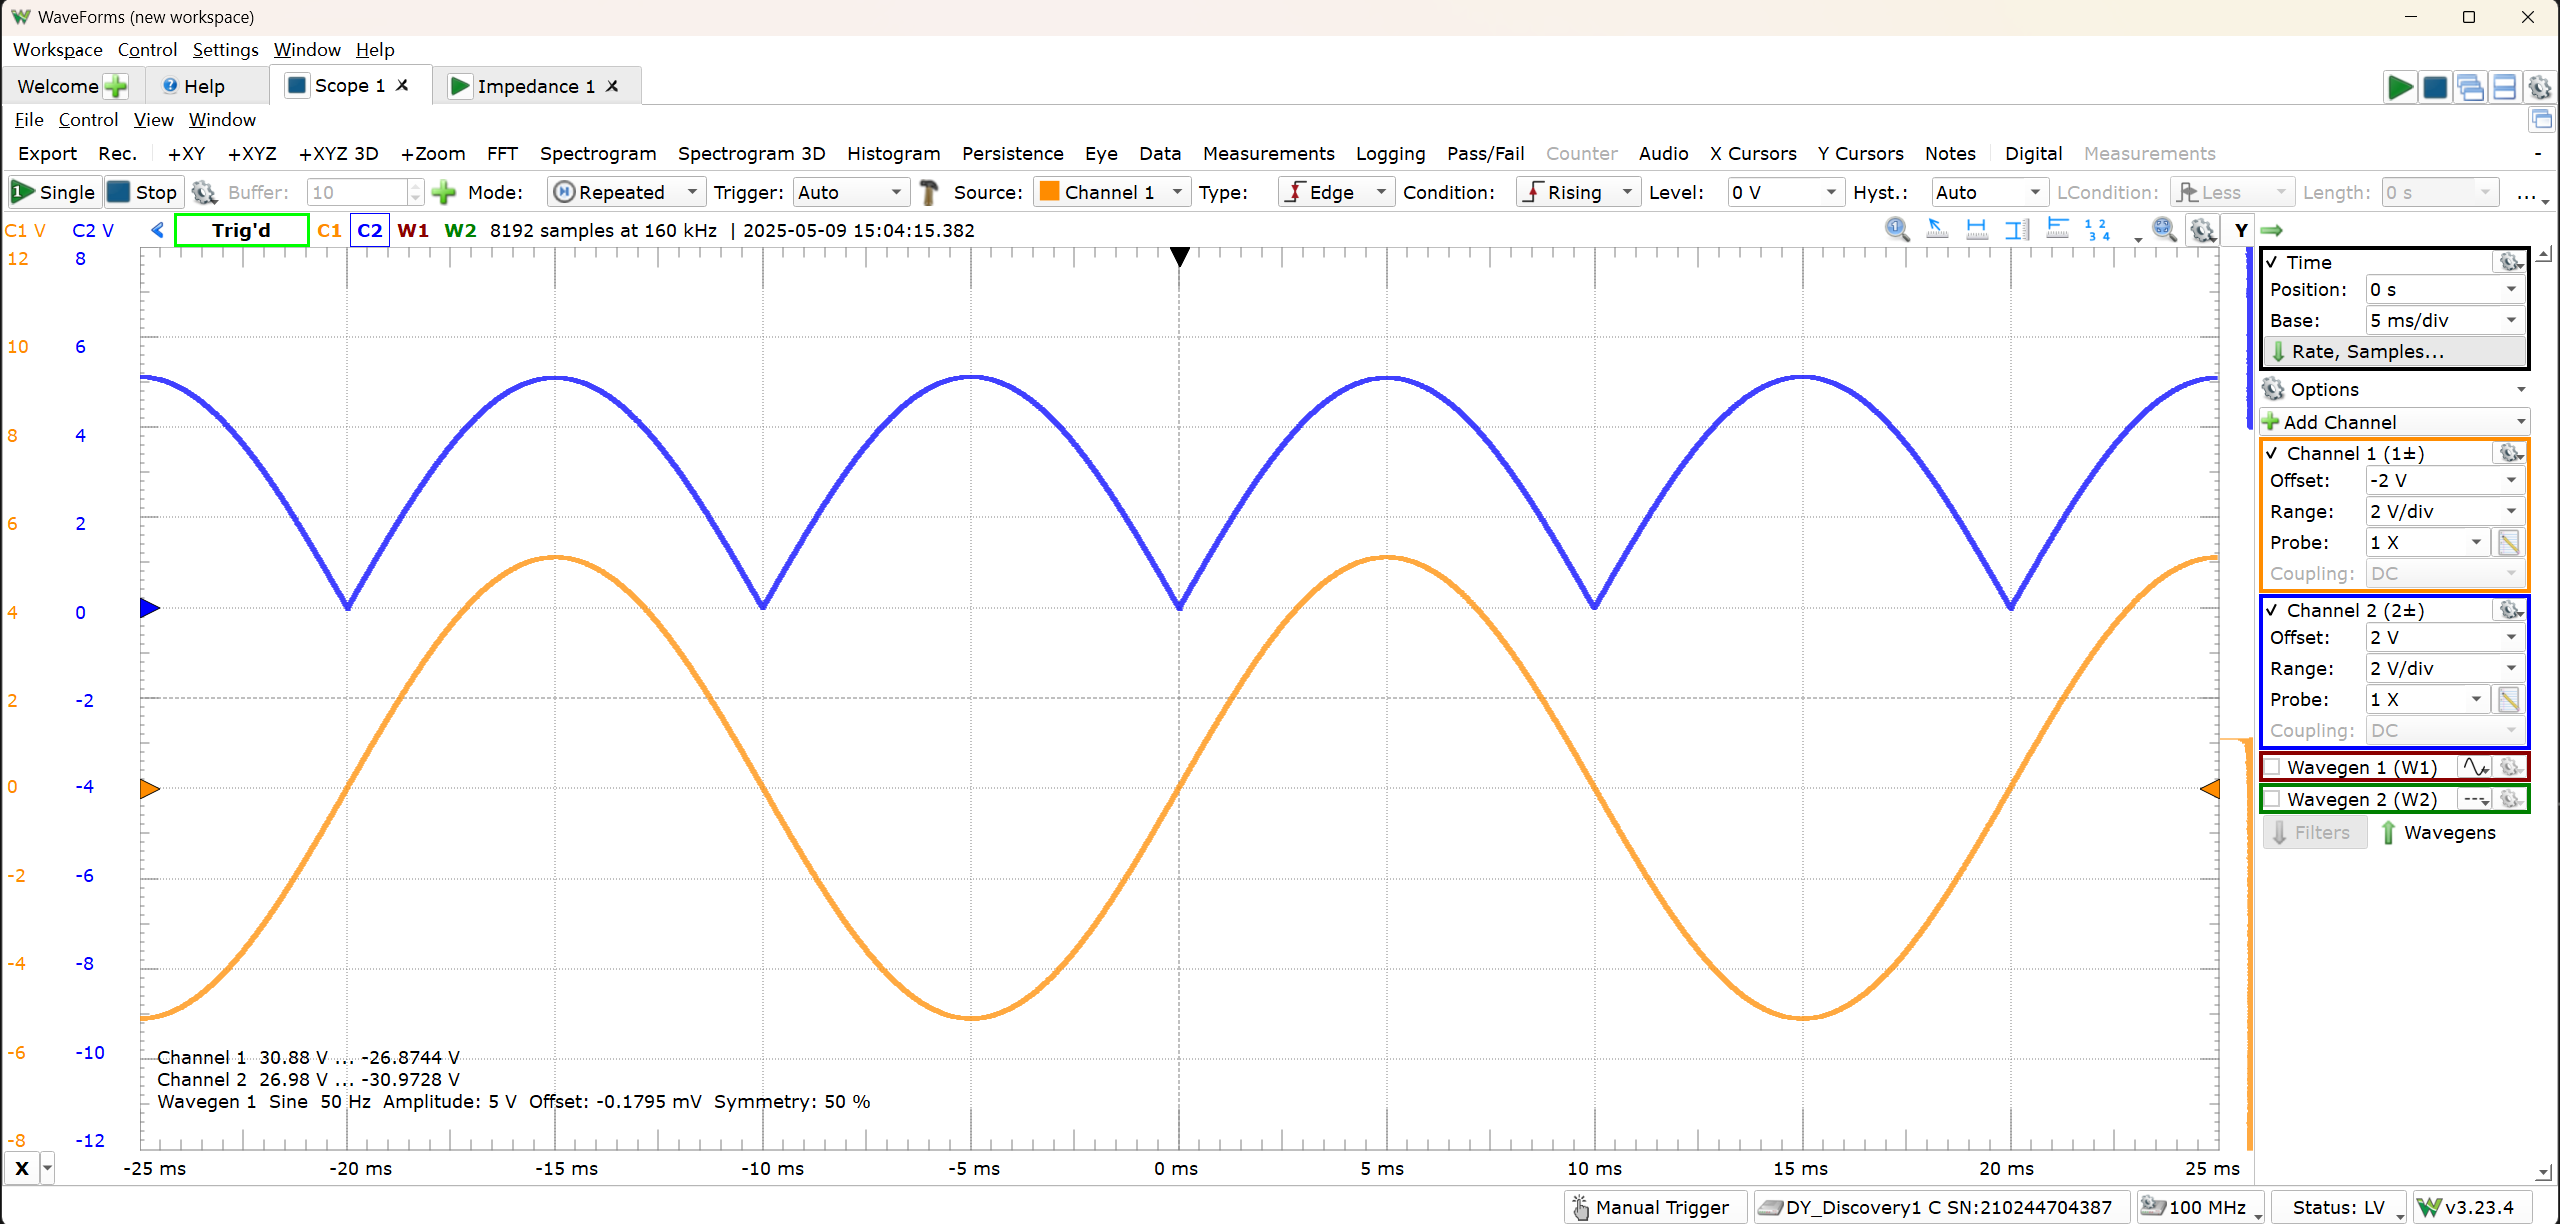
\includegraphics[width=\columnwidth]{LCE-05-精密整流/assets/1N4148/1N4148 input-output waveform (50 Hz) 2.png}
    \caption{精密整流电路 (diode 1: 1N4148),输入输出波形 (sine input, 5 Vamp @ 50 Hz),错位显示; CH1 (orange) input, CH2 (blue) output}
\end{figure}

\begin{figure}[H]\centering
    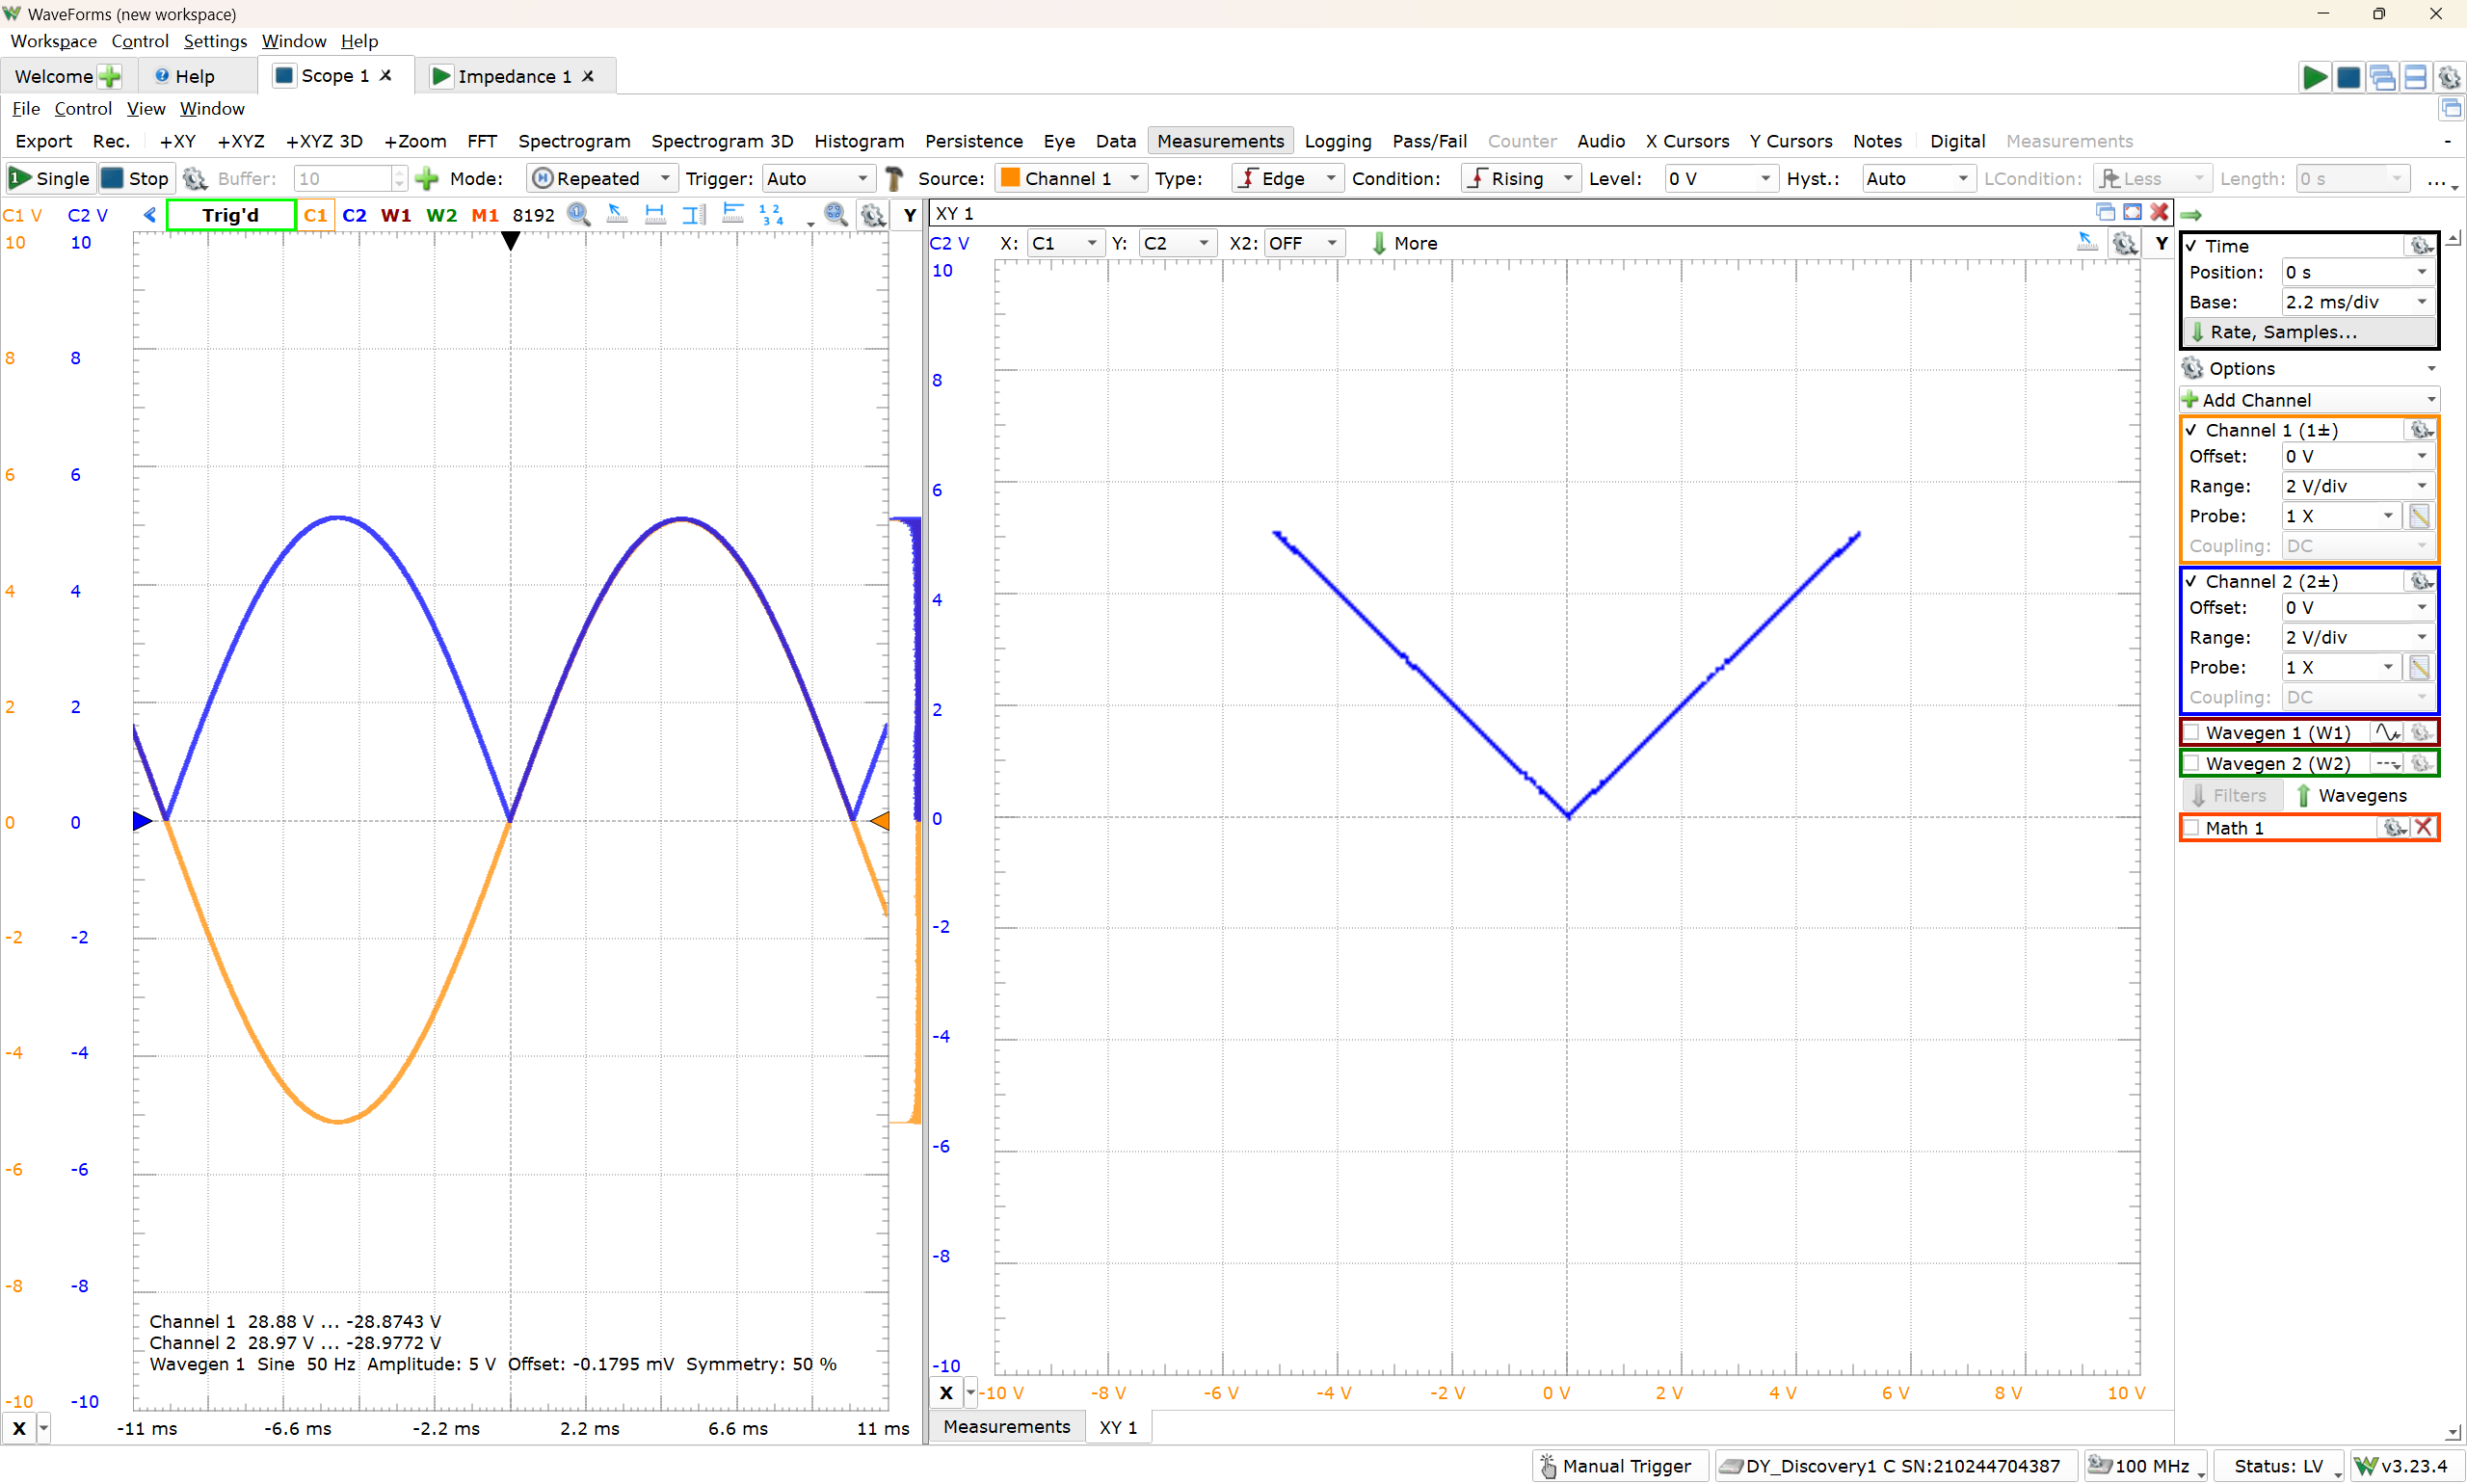
\includegraphics[width=\columnwidth]{LCE-05-精密整流/assets/1N4148/1N4148 input-output waveform (50 Hz) 3.png}
    \caption{精密整流电路 (diode 1: 1N4148),输入输出波形 (sine input, 5 Vamp @ 50 Hz), X-Y 显示; CH1 (orange) input, CH2 (blue) output}
\end{figure}
\vspace*{-3mm}
从图中可以看到,电路正常工作,输出信号与输入信号的绝对值基本相符。进一步,我们可以计算出输出波形的平均值 $(V_{out})_{mean}$ 和相对整流误差 $\eta$:
\begin{gather}
(V_{out})_{mean} = \frac{1}{T}\int_0^T V_{out}(t) dt,\quad 
\eta = \frac{V_{out} - \mathrm{abs}(V_{in})}{\mathrm{Amplitude}}\times 100 \,\% = \frac{V_{out} - \mathrm{abs}(V_{in})}{5 \ \mathrm{V}}\times 100 \,\%
\end{gather}


\noindent 这两个量可以分别利用 WaveForms 的 Measurement 功能和 Math 功能计算得到,结果如图 \ref{1N4148 input-output waveform (50 Hz) 1} 所示:
\begin{gather}
(V_{out})_{mean} = 3.2674 \ \mathrm{V},\quad
\eta \in (0.0\, \%, +0.5\, \%)
\end{gather}
\vspace*{-3mm}
\begin{figure}[H]\centering
    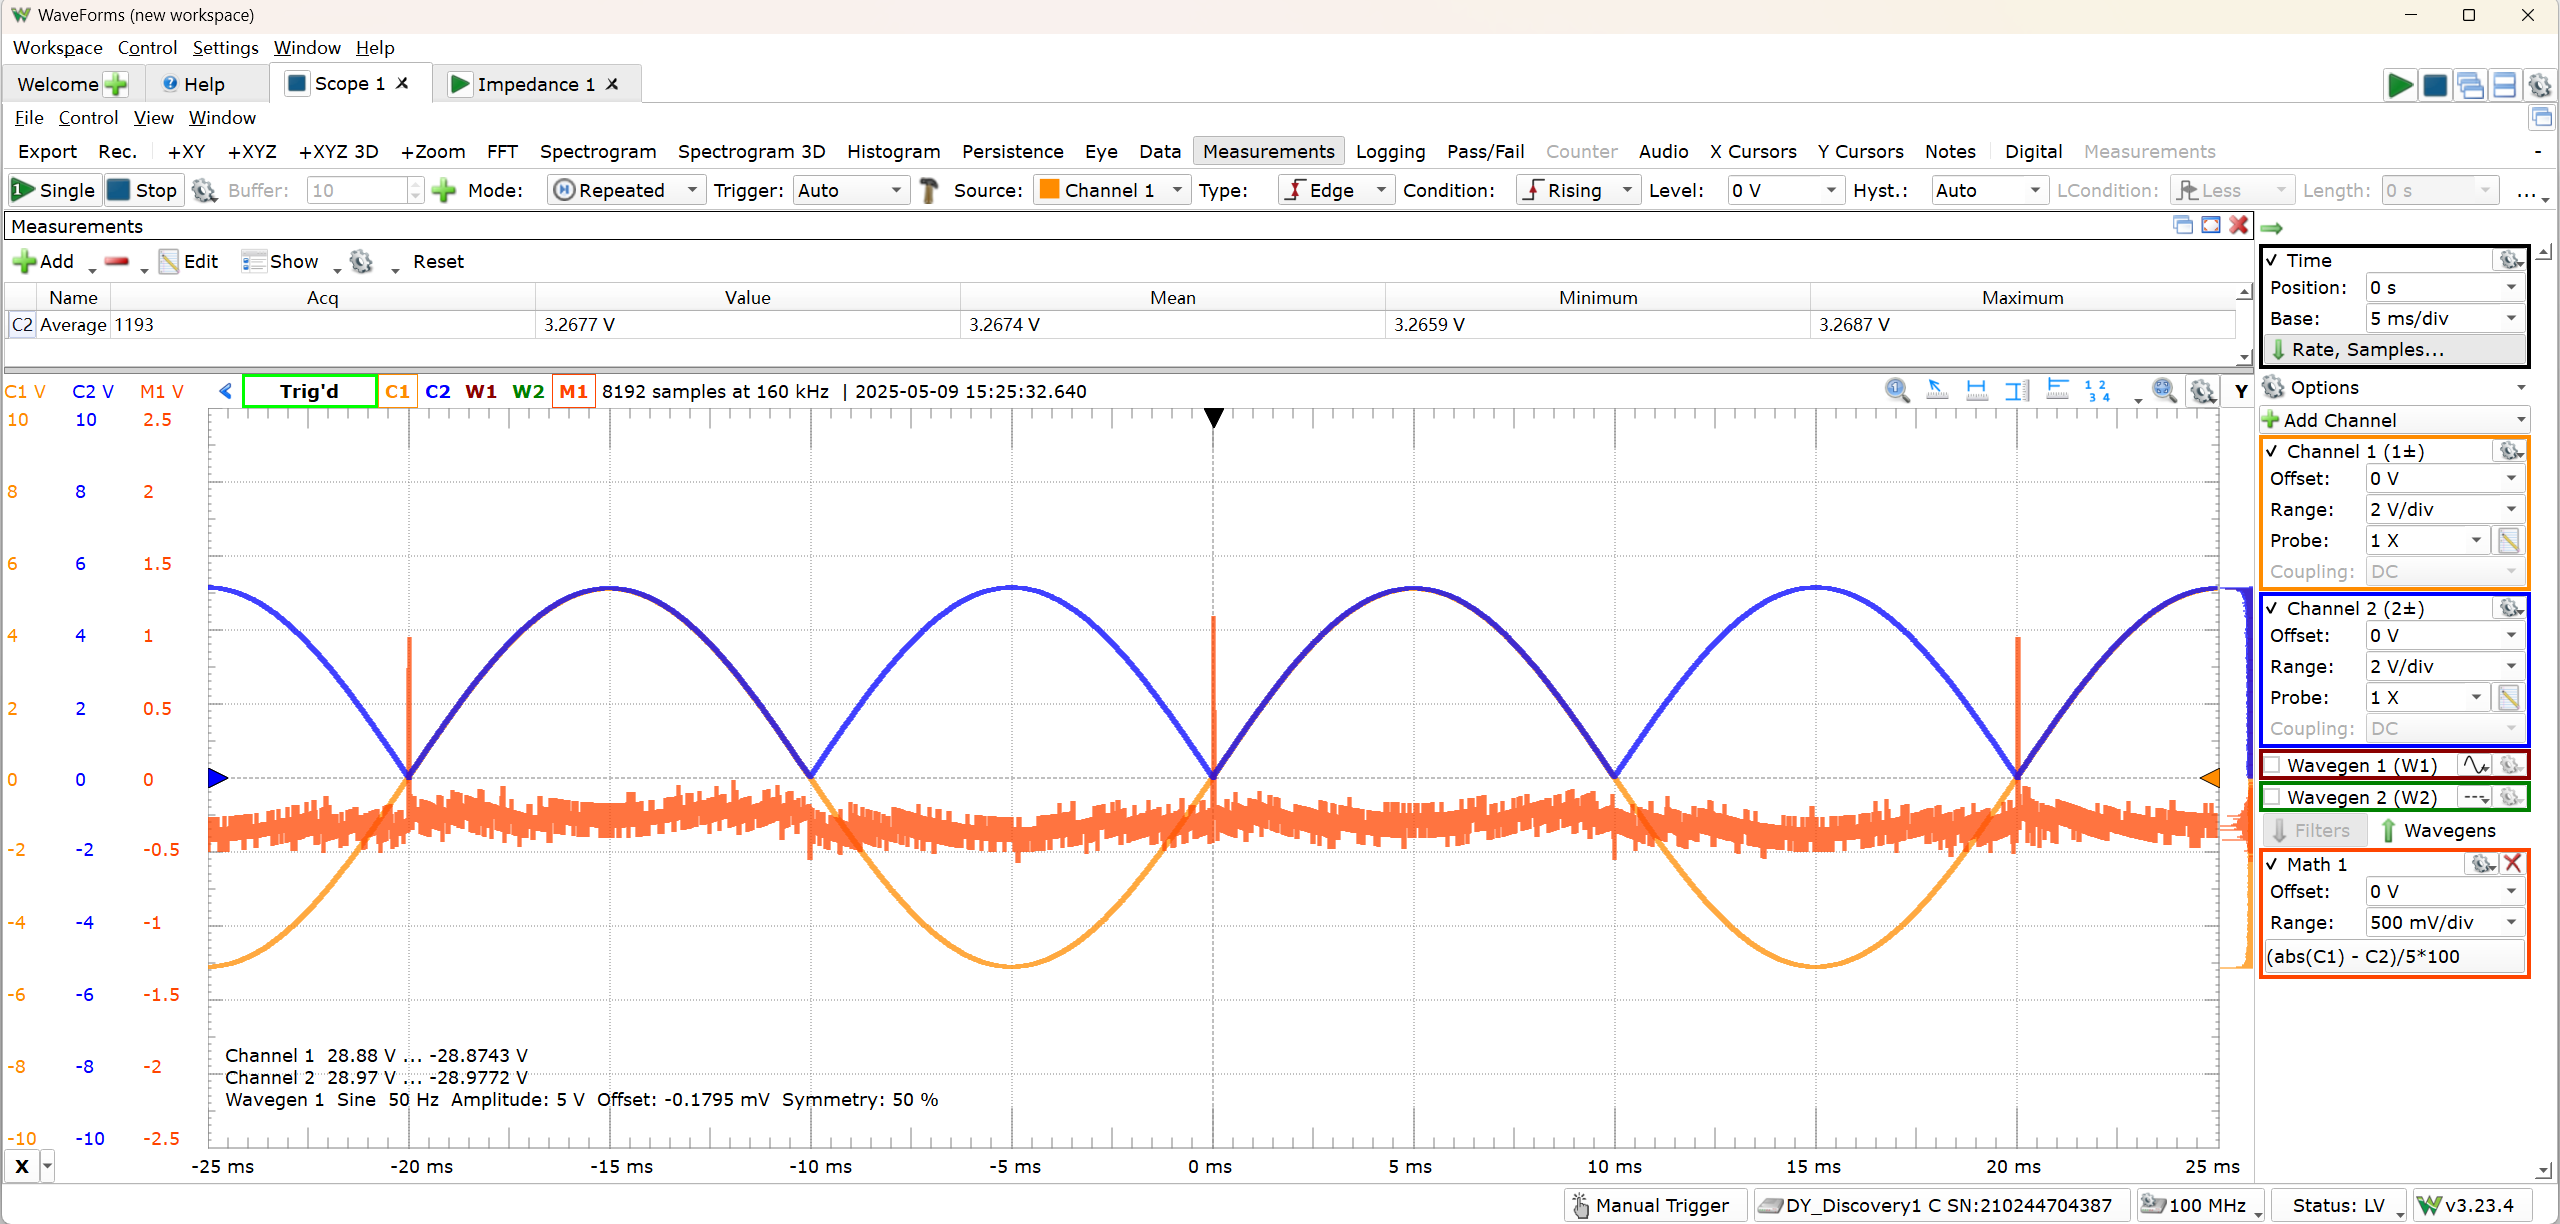
\includegraphics[width=\columnwidth]{LCE-05-精密整流/assets/1N4148/1N4148 input-output waveform (50 Hz) 1.png}
    \caption{精密整流电路 (diode 1: 1N4148),输入输出波形 (sine input, 5 Vamp @ 50 Hz),计算输出平均值和相对整流误差; CH1 (orange) input, CH2 (blue) output, M1 (red) relative error}
    \label{1N4148 input-output waveform (50 Hz) 1}
\end{figure}

\newpage
\vspace*{-13mm}
\subsubsection{测量最高工作频率与频率响应}

随着输入频率的升高,输出波形首先会在 0 V 转折点出现失真,频率进一步升高,失真明显,电路无法正常工作。如何评判电路(在此运放和此二极管下)的最高工作频率呢?我们利用输出波形的平均值来判断。具体而言,假设 50 Hz 时输出波形的平均值为 $(V_{out})_{mean}^{\mathrm{50\ Hz}}$,当频率升高到某个值 $f_{max}$ 时,输出平均值 $(V_{out})_{mean}^{f_{max}}$ 降低了 1 \%,也即 $(V_{out})_{mean}^{f_{max}} = 99\,\% \times (V_{out})_{mean}^{\mathrm{50\ Hz}}$ 时,我们便认为电路达到了最高工作频率 $f_{max}$。

设置输入信号为 5 Vamp, 由图 \ref{1N4148 input-output waveform (50 Hz) 1} 知道 $(V_{out})_{mean}^{\mathrm{50\ Hz}} = 3.2674 \ \mathrm{V}$, 那么最高频率处有 $(V_{out})_{mean}^{f_{max}} = 3.2347 \ \mathrm{V}$。不断调整输入频率,直到输出平均值达到 3.2347 V 左右,得到最高工作频率为 20 kHz, 如下图所示:
\begin{gather}
f_{max} = 20 \ \mathrm{kHz},\quad (V_{out})_{mean}^{20 \ \mathrm{kHz}} = 3.2343 \ \mathrm{V}
\end{gather}\vspace*{-7mm}
\begin{figure}[H]\centering
    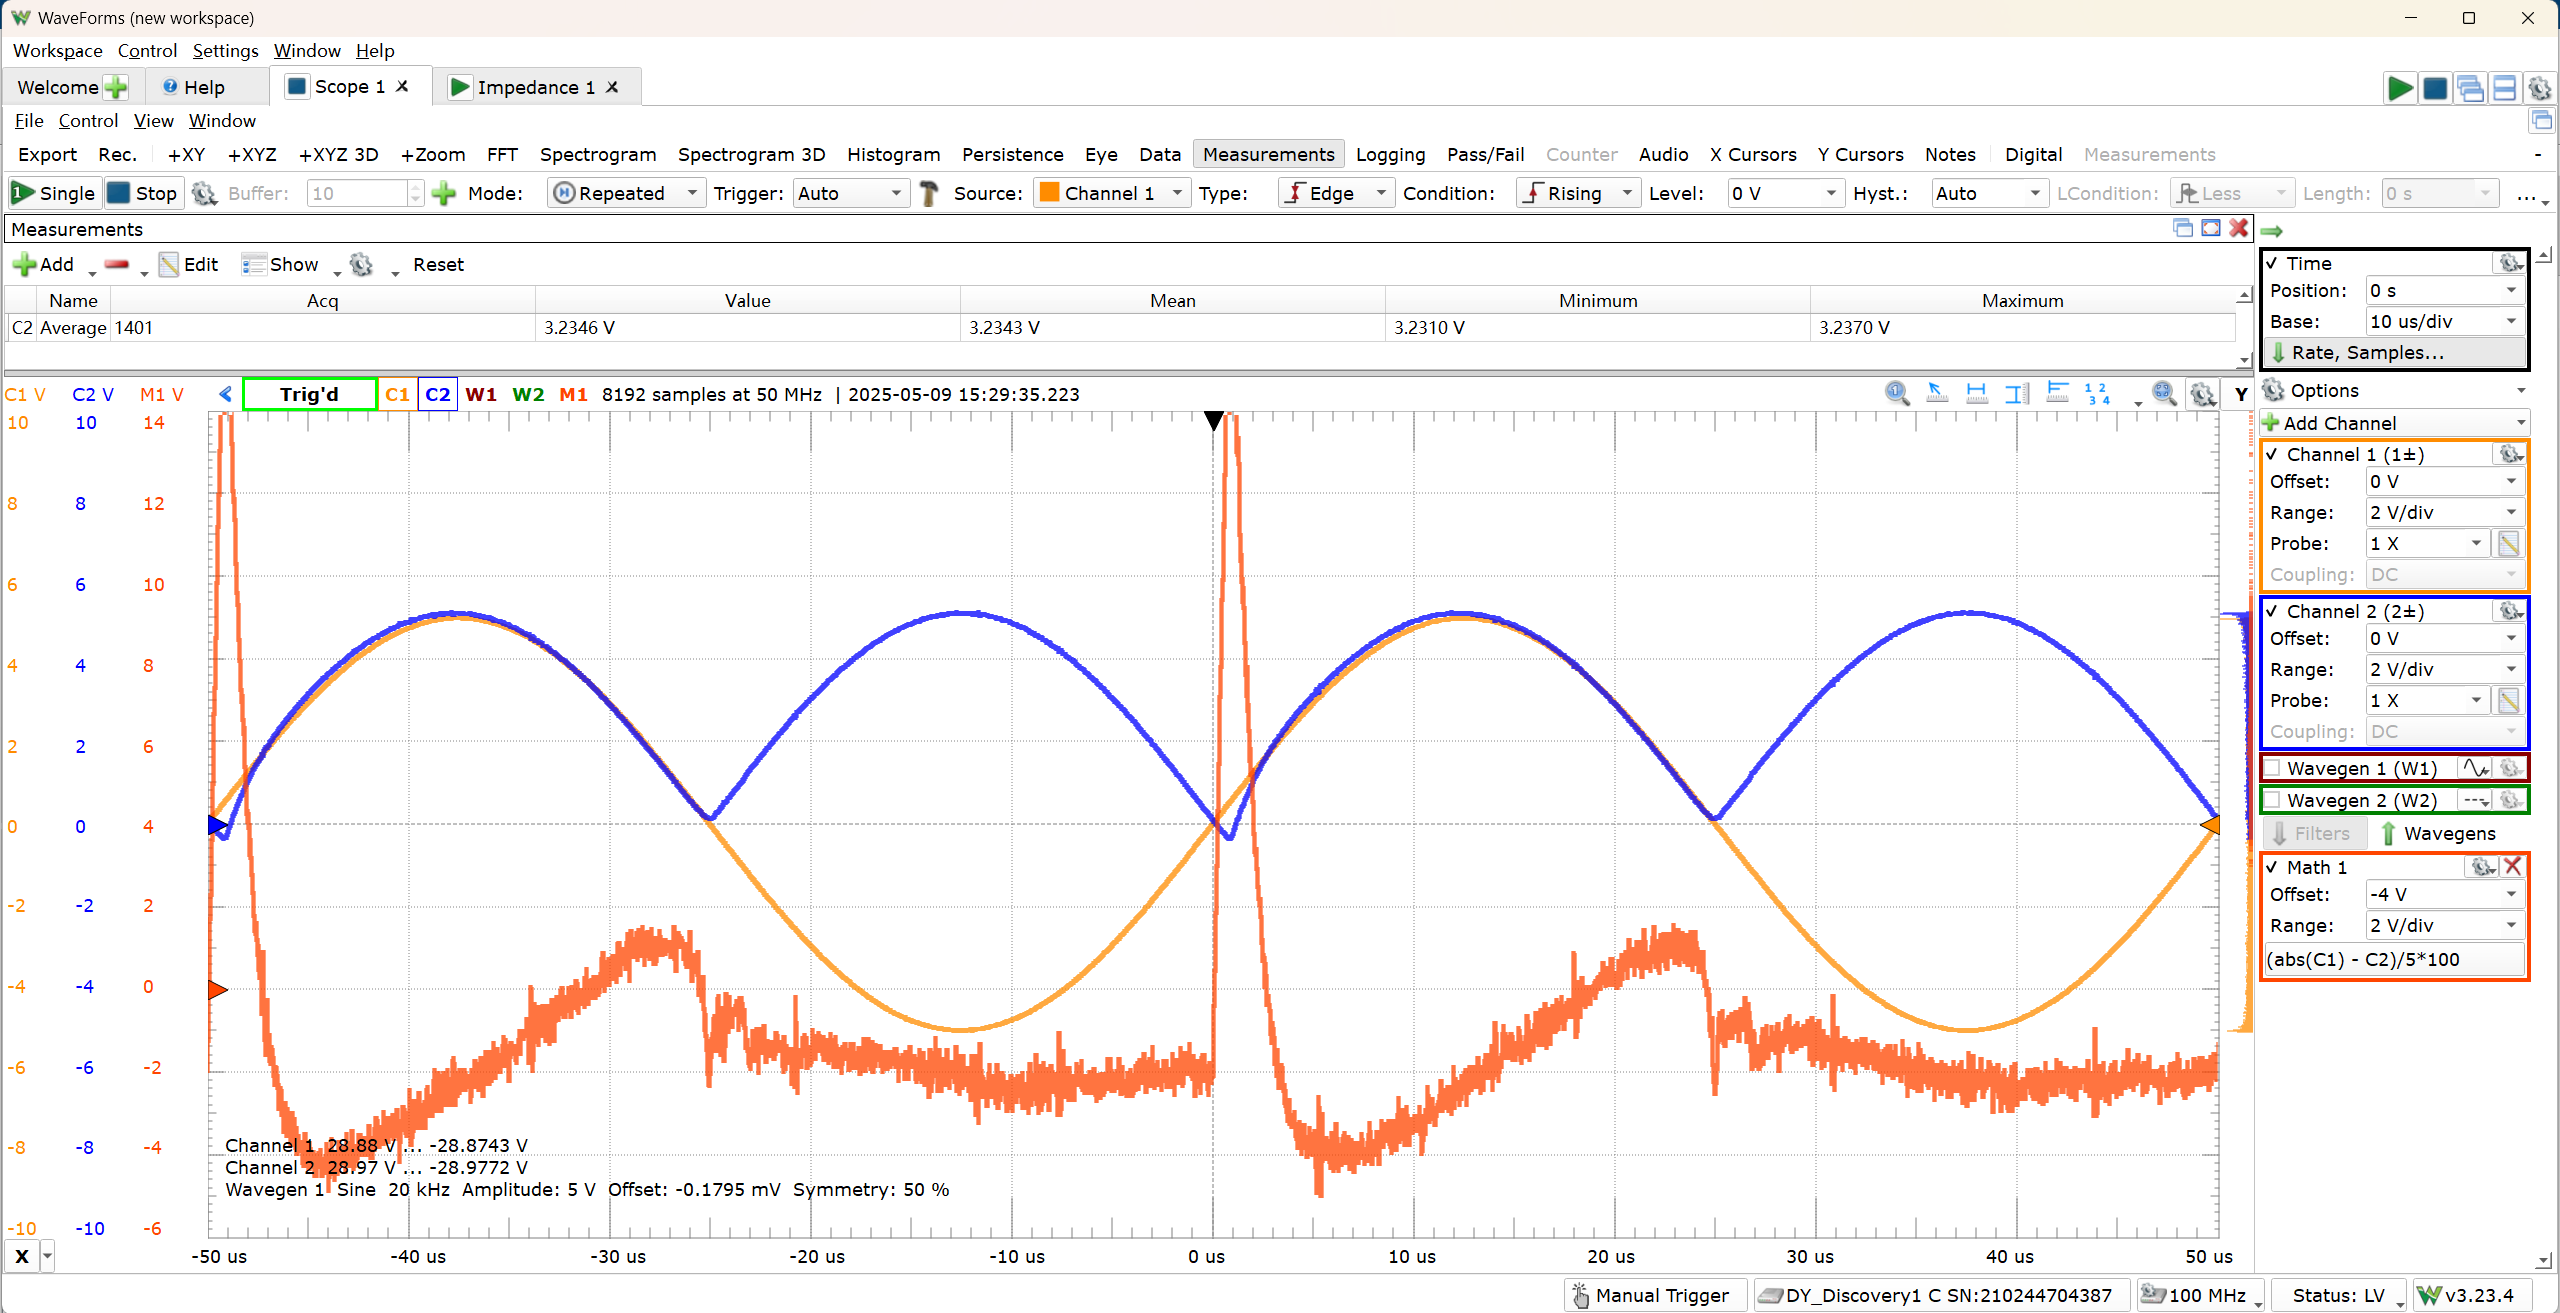
\includegraphics[width=\columnwidth]{LCE-05-精密整流/assets/1N4148/1N4148 input-output waveform (max 20 kHz) with error and mean.png}
    \caption{精密整流电路 (diode 1: 1N4148),最高工作频率 (sine input, 5 Vamp),$f = 20 \ \mathrm{kHz}$, $(V_{out})_{mean} = 3.2343 \ \mathrm{V}$; CH1 (orange) input, CH2 (blue) output, M1 (red) relative error}
\end{figure}



\vspace*{-3mm}
需要注意的是,按上面的方法测量得到的 $f_{max}$ 不仅与运放、二极管有关,还与输入信号幅度有关。我们可以通过测量不同输入幅度下的频响曲线来验证这一点:
\vspace*{-7mm}
\begin{figure}[H]\centering
    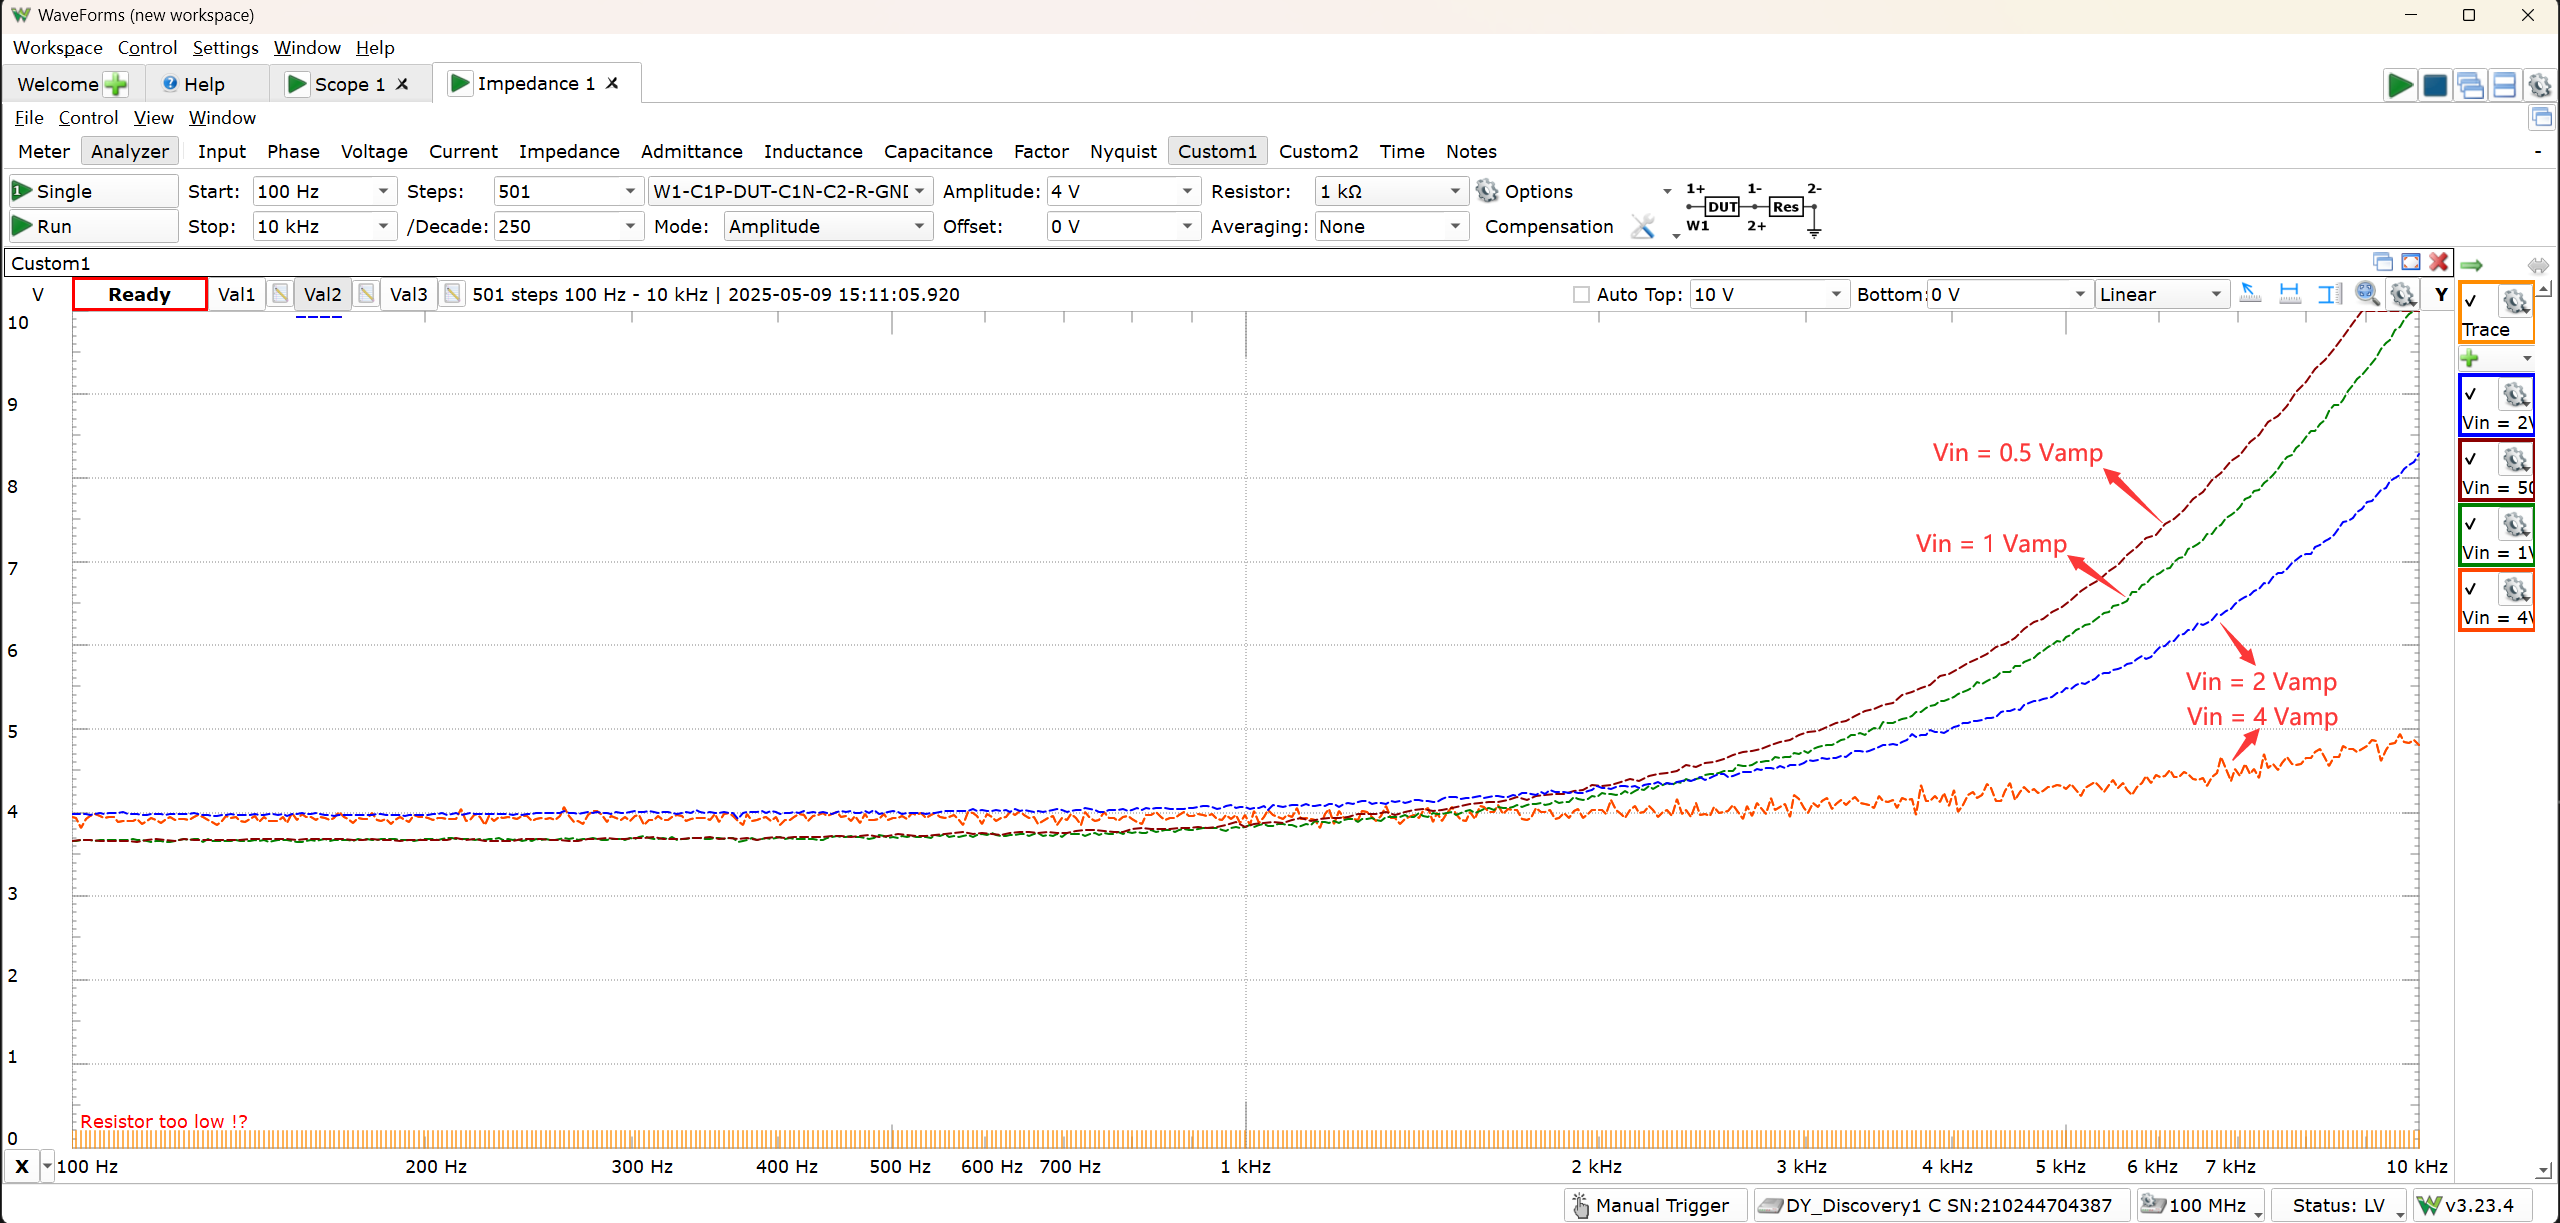
\includegraphics[width=\columnwidth]{LCE-05-精密整流/assets/1N4148/1N4148 frequency response.png}
    \caption{精密整流电路 (diode 1: 1N4148),频率响应曲线 (sine input, 0.5 Vamp $\sim$ 4 Vamp)}
\end{figure}

从上图可以看出,输入信号幅度越大,波形失真越不明显,最高工作频率越高。这与我们的直觉相符。

\subsubsection{测量输出平均值关于输入幅度的线性度}

现在,我们来考察输入幅度与输出信号平均值之间的线性关系,实验测得数据如下:

%\begin{table}[H]\centering
%    %\renewcommand{\arraystretch}{1.5} % 调整行间距
%    %\setlength{\tabcolsep}{1.5mm} % 调整列间距
%    \caption{输入幅度与输出信号平均值之间的关系 (input sine wave @ 50 Hz)}
%    \label{输入幅度与输出信号平均值之间的关系}
%\begin{tabular}{cccccccccc}\toprule
%    Input amplitude (V) & Mean value of output signal (V)  \\
%    \midrule
%    5.0	& 3.2680 \\
%    4.5	& 2.9419 \\
%    4.0	& 2.6175 \\
%    3.7	& 2.4219 \\
%    3.4	& 2.2269 \\
%    3.1	& 2.0314 \\
%    2.8	& 1.8358 \\
%    2.5	& 1.6408 \\
%    2.2	& 1.4454 \\
%    1.9	& 1.2505 \\
%    1.6	& 1.0425 \\
%    1.3	& 0.8472 \\
%    1.0	& 0.6526 \\
%    \bottomrule
%\end{tabular}
%\end{table}


\begin{table}[H]\centering
    %\renewcommand{\arraystretch}{1.5} % 调整行间距为 1.5 倍
    %\setlength{\tabcolsep}{1.5mm} % 调整列间距
    \caption{输入幅度与输出信号平均值之间的关系 (input sine wave @ 50 Hz)}
    \label{输入幅度与输出信号平均值之间的关系}

\resizebox{\linewidth}{!}{   % 设置宽度为 \linewidth 等比例缩放
\begin{tabular}{ccccccccccccccccccccc}\toprule
    Input amplitude (V) & 5.0 & 4.5 & 4.0 & 3.7 & 3.4 & 3.1 & 2.8 & 2.5 & 2.2 & 1.9 & 1.6 & 1.3 & 1.0 \\
    \midrule
    Mean value of output signal (V) &  3.2680 & 2.9419 & 2.6175 & 2.4219 & 2.2269 & 2.0314 & 1.8358 & 1.6408 & 1.4454 & 1.2505 & 1.0425 & 0.8472 & 0.6526 \\
    \bottomrule
\end{tabular}
}\end{table}

用函数 $y = ax$ 对数据进行拟合,观察线性度:
\begin{figure}[H]\centering
    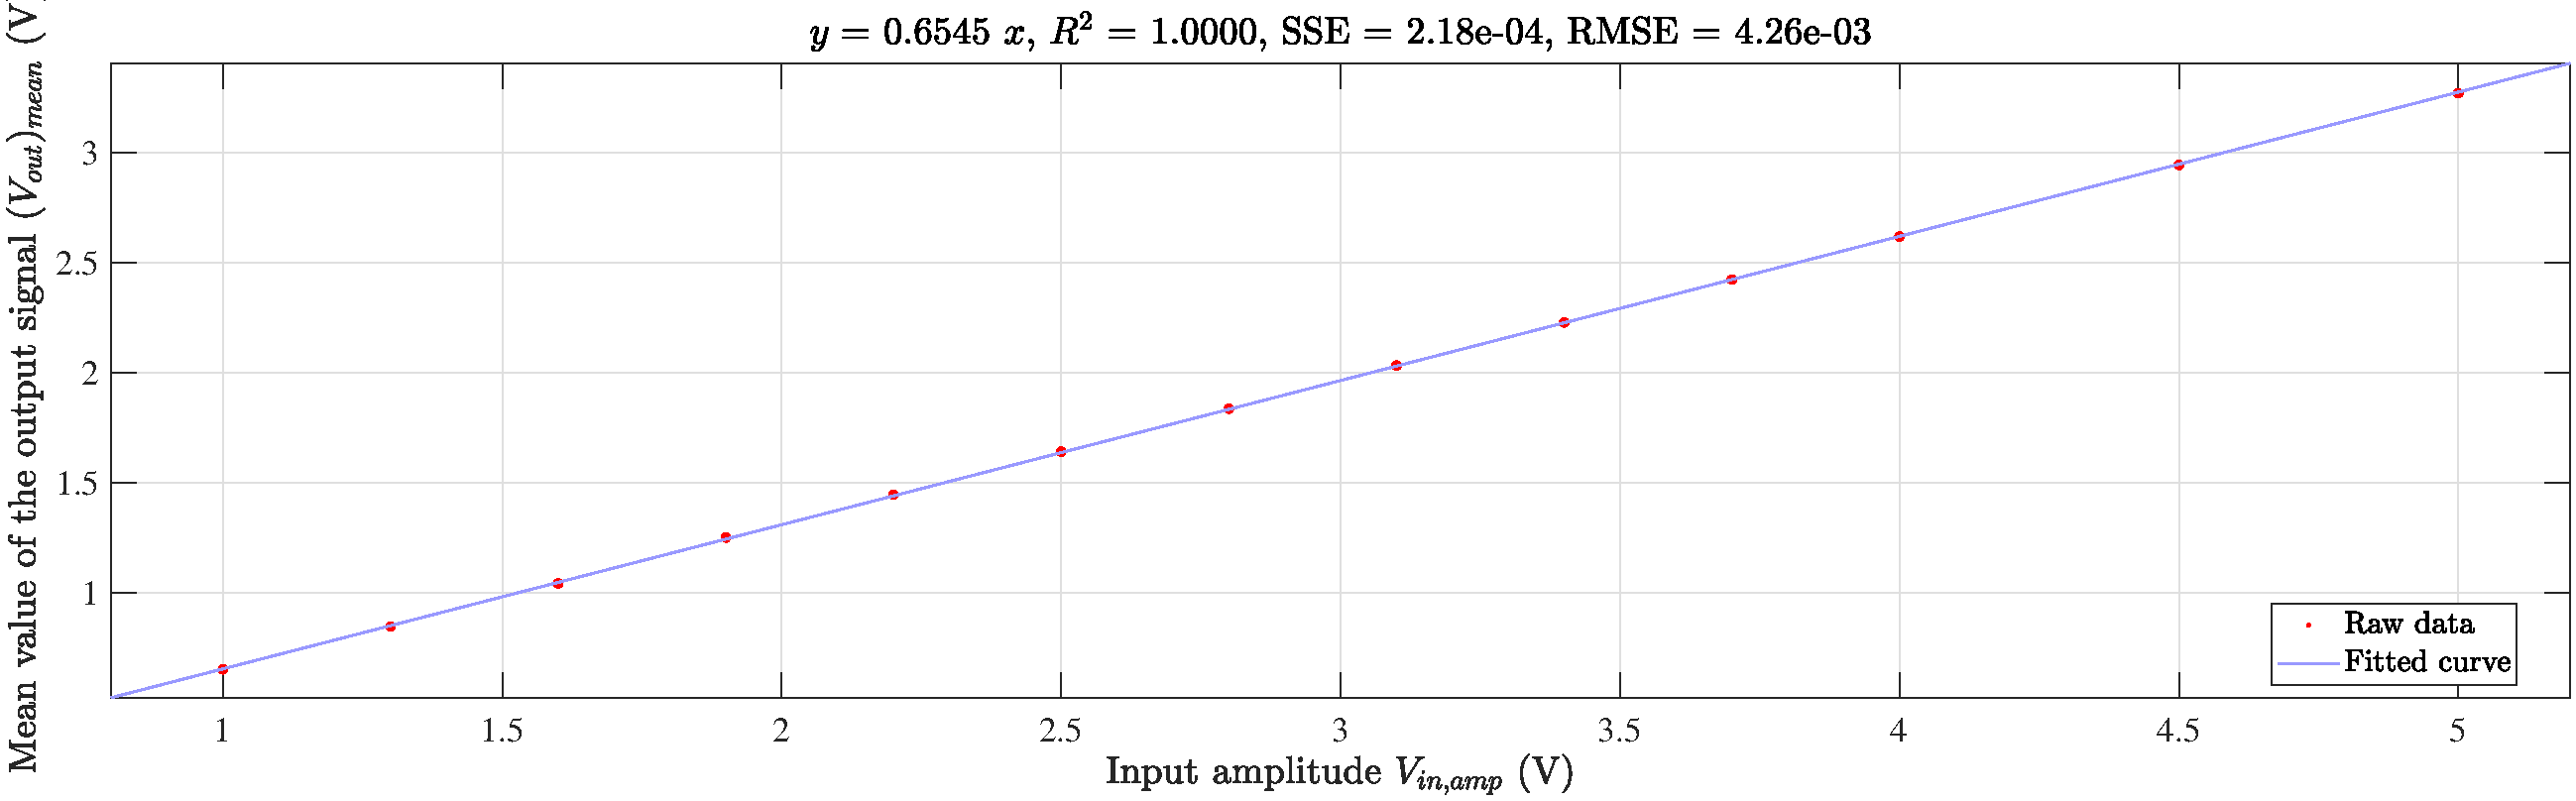
\includegraphics[width=\columnwidth]{LCE-05-精密整流/assets/1N4148/linearity.pdf}
    \caption{正比例拟合输入幅度与输出信号平均值 (input sine wave @ 50 Hz)}
\end{figure}

从上图可以看出,$R^2 = 1.000$,输入输出线性度极好。

\subsubsection{对比整流电路与 AD637 RMS 电路输出响应}

下面,我们来对比不同输入信号下,整流电路(绝对值电路)输出信号的平均值与 AD637 RMS 电路输出信号之间的差异。设置输入信号都为 5 Vamp @ 1 kHz, 特别地, burst 模式下设置为 sine wave ($f = 1 \ \mathrm{kHz},\ T = 10 \ \mathrm{ms}$), 也即 D = 0.1 (1 ms / 10 ms)。实验测得数据如下:

\begin{table}[H]\centering
    %\renewcommand{\arraystretch}{1.5} % 调整行间距
    %\setlength{\tabcolsep}{1.5mm} % 调整列间距
    \caption{绝对值电路与 AD637 RMS 电路输出响应对比}
    \label{绝对值电路与 AD637 RMS 电路输出响应对比}
\begin{tabular}{cccccccccc}\toprule
    Waveform & sine  & triangular & burst \\
    \midrule
    Mean value of the rectifier circuit & 3.2428 V & 2.5476 V & 0.3416 V \\
    Output voltage of AD637 RMS circuit & 3.5630 V & 2.9091 V & 1.1255 V \\
    \bottomrule
\end{tabular}
\end{table}

后两种信号 (triangular, burst) 的输入输出波形如下图所示:

\begin{figure}[H]\centering
    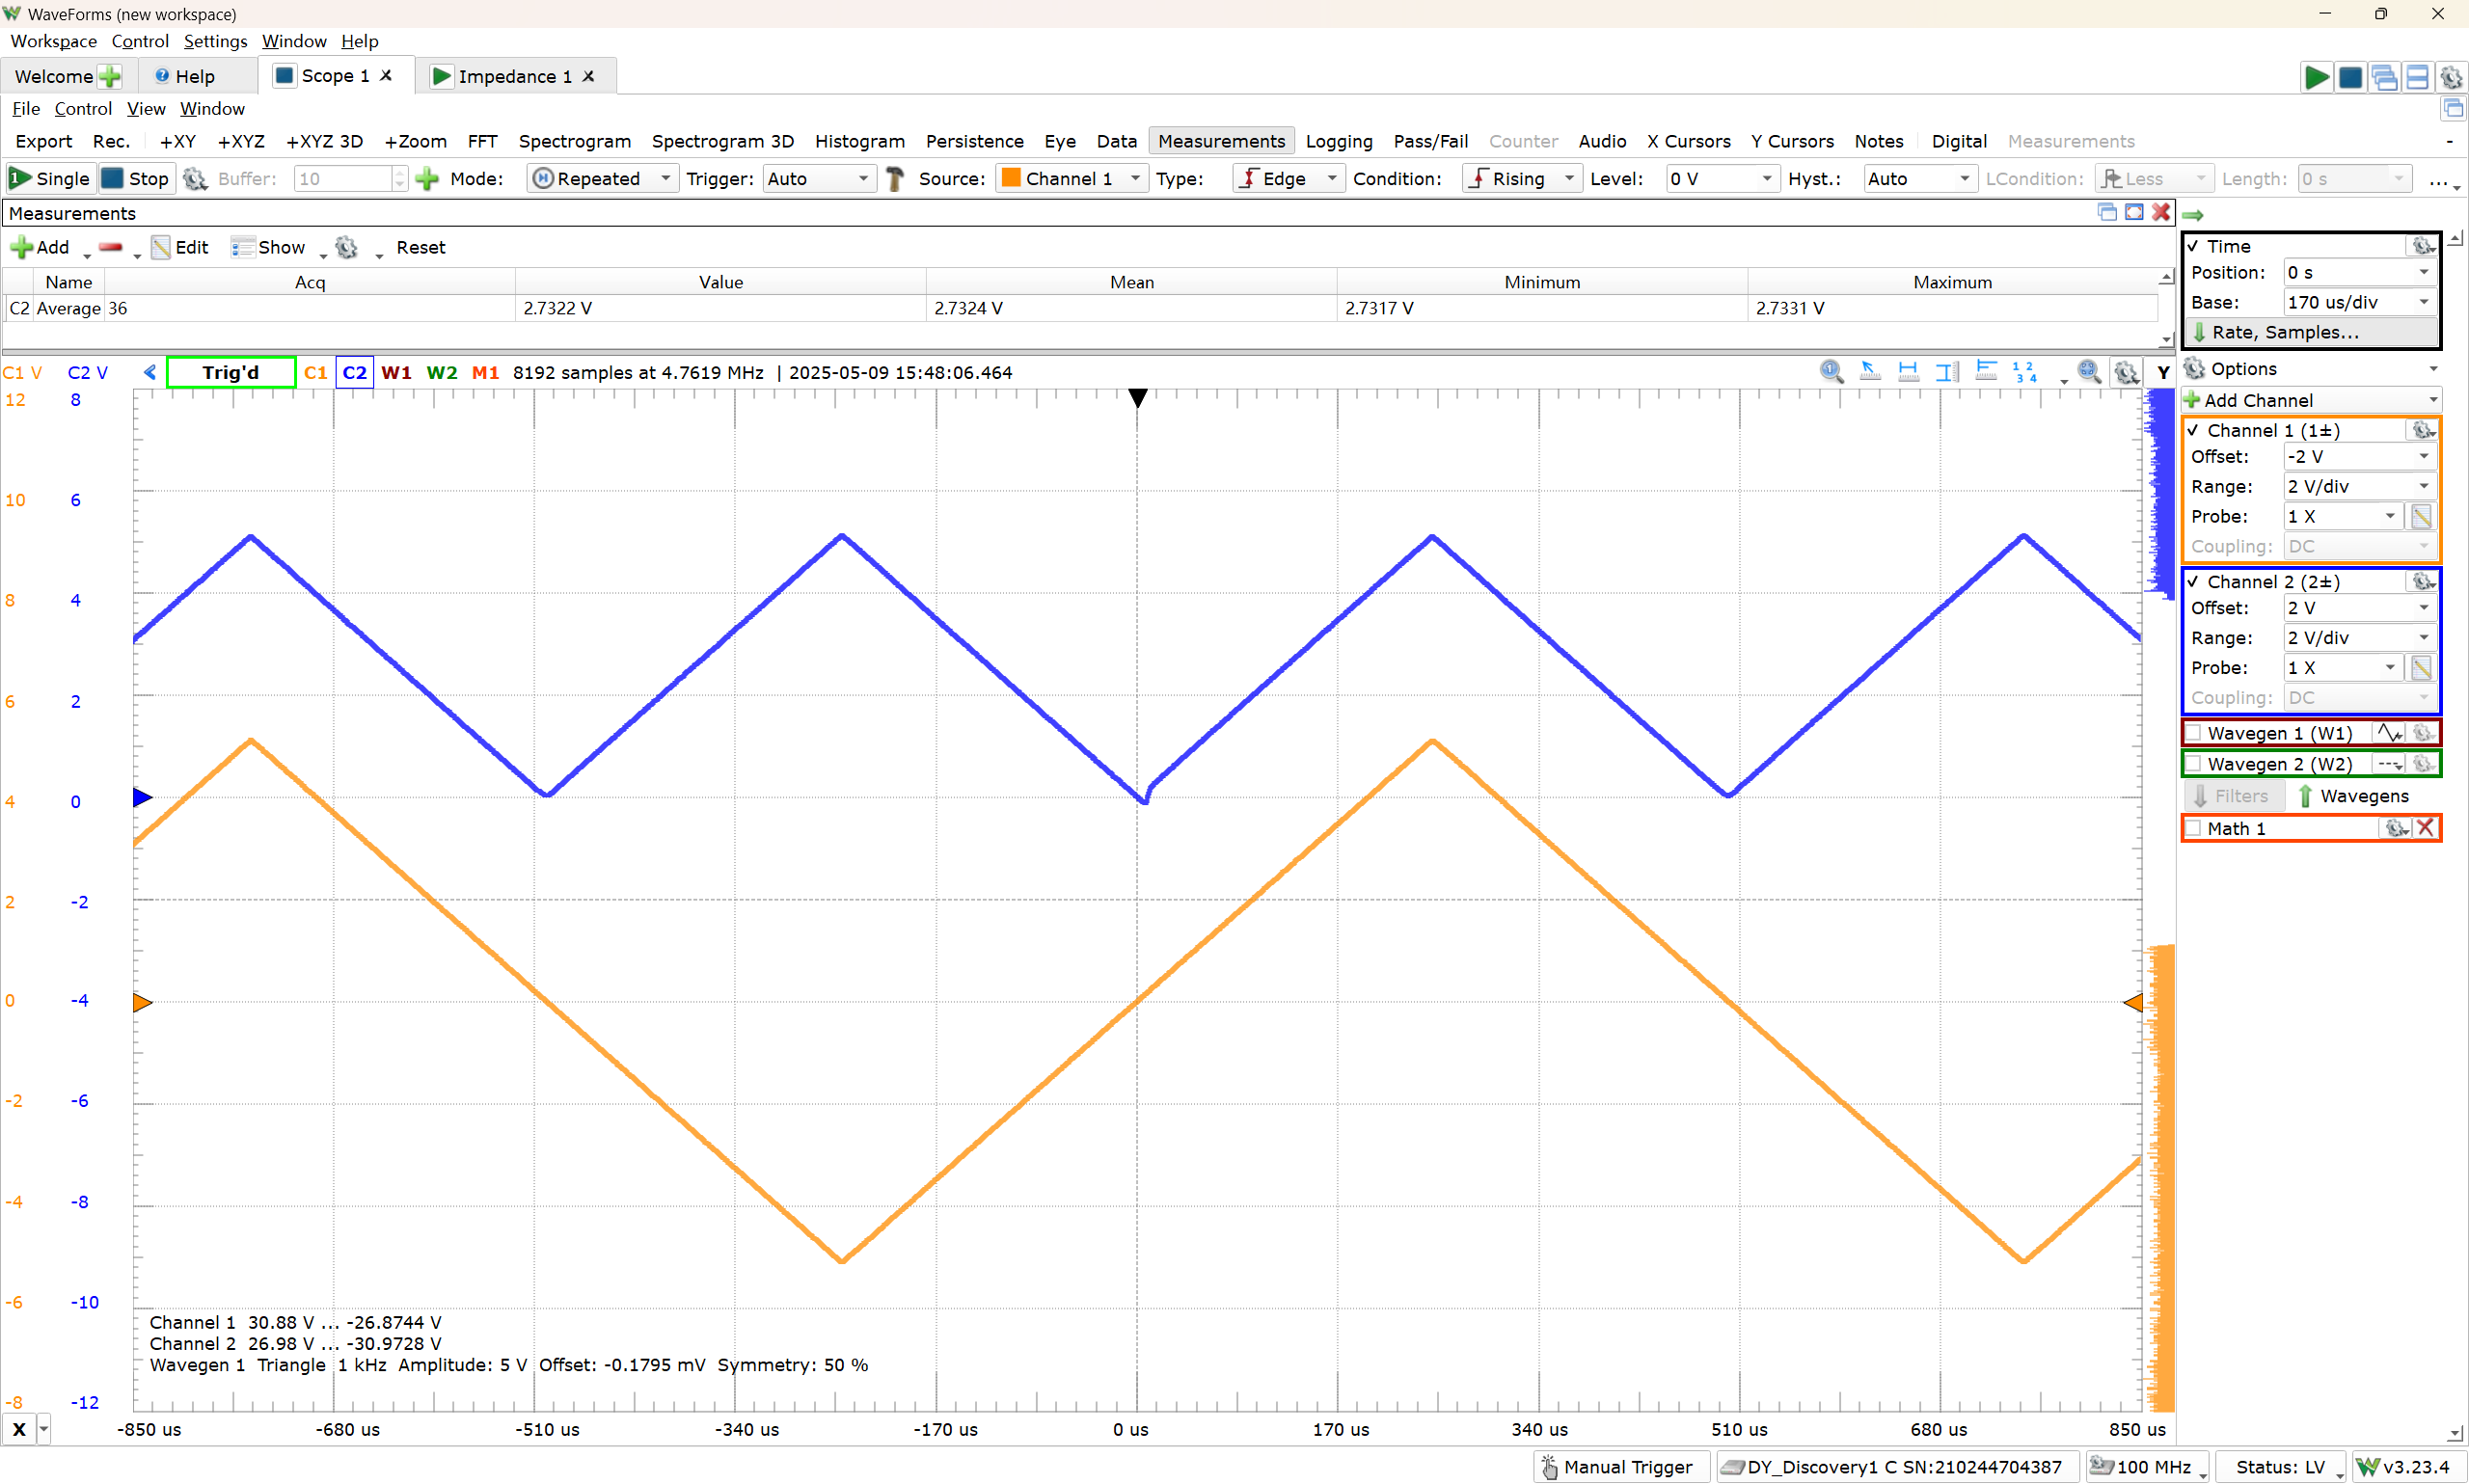
\includegraphics[width=\columnwidth]{LCE-05-精密整流/assets/1N4148/1N4148 triangular wave (1 kHz) (2).png}
    \caption{精密整流电路 (diode 1: 1N4148),输入输出波形 (triangular input, 5 Vamp @ 1 kHz),错位显示; CH1 (orange) input, CH2 (blue) output}
\end{figure}

\begin{figure}[H]\centering
    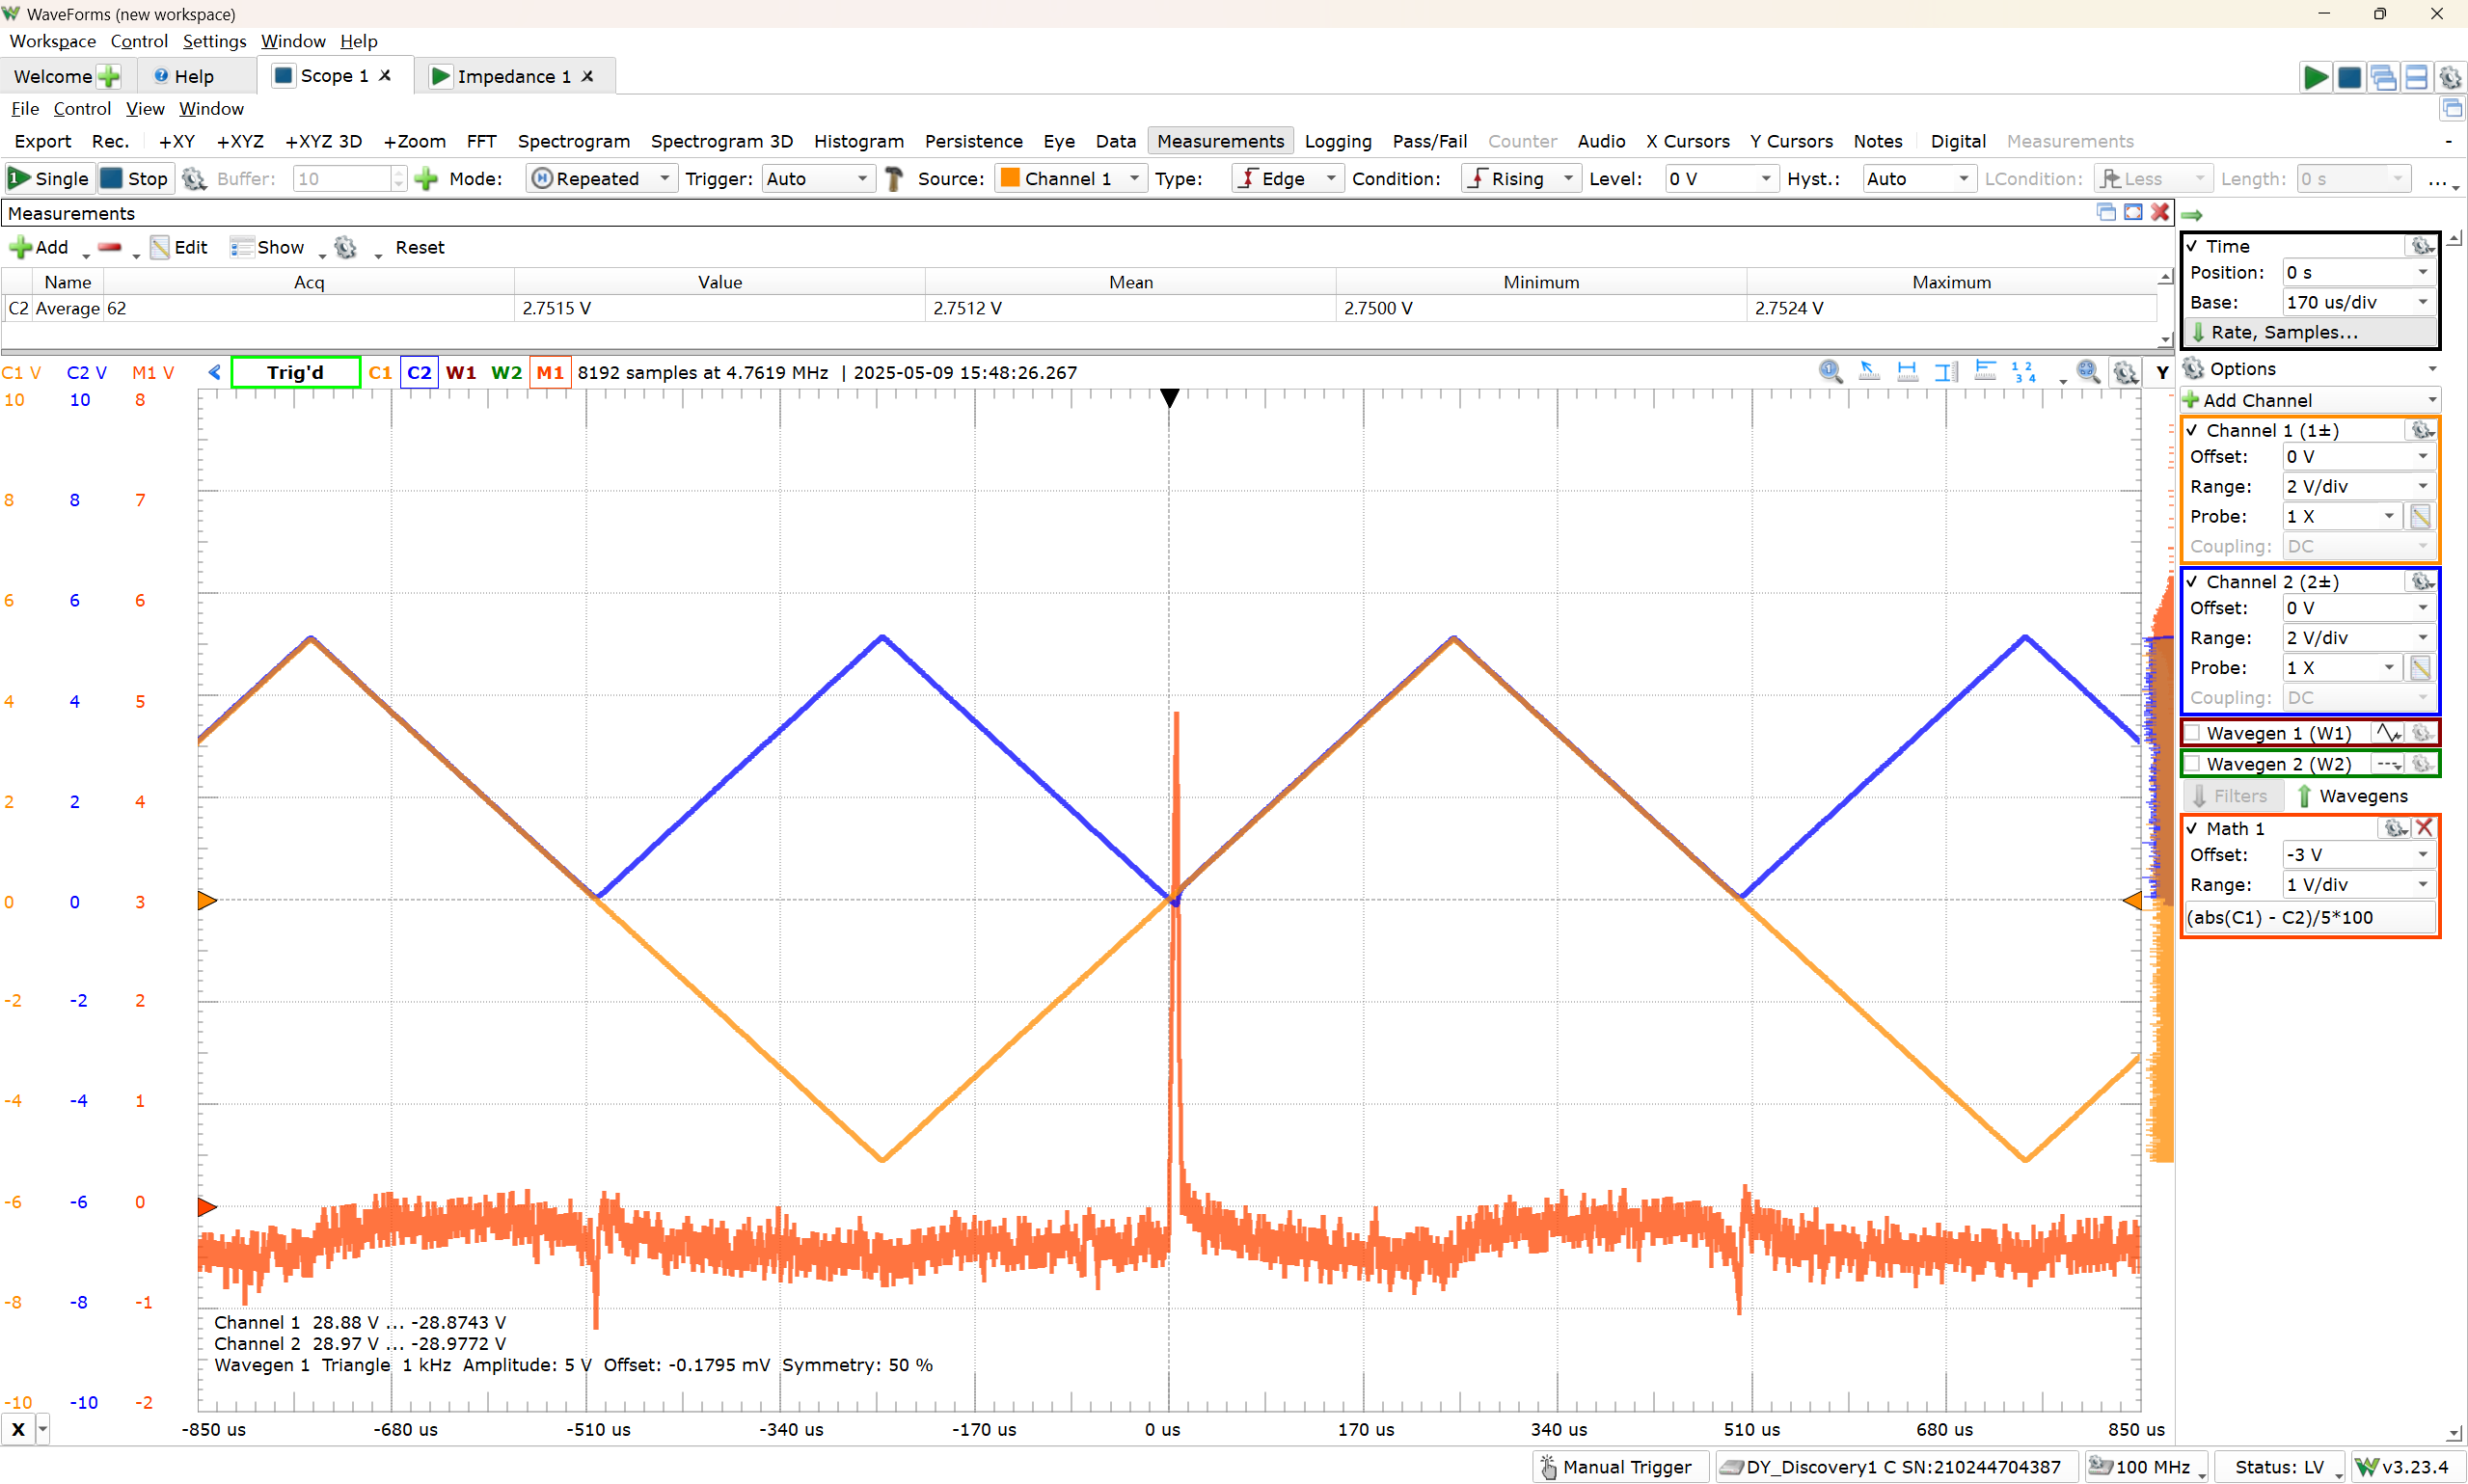
\includegraphics[width=\columnwidth]{LCE-05-精密整流/assets/1N4148/1N4148 triangular wave (1 kHz).png}
    \caption{精密整流电路 (diode 1: 1N4148),输入输出波形 (triangular input, 5 Vamp @ 1 kHz),计算输出平均值和相对整流误差}
\end{figure}

\begin{figure}[H]\centering
    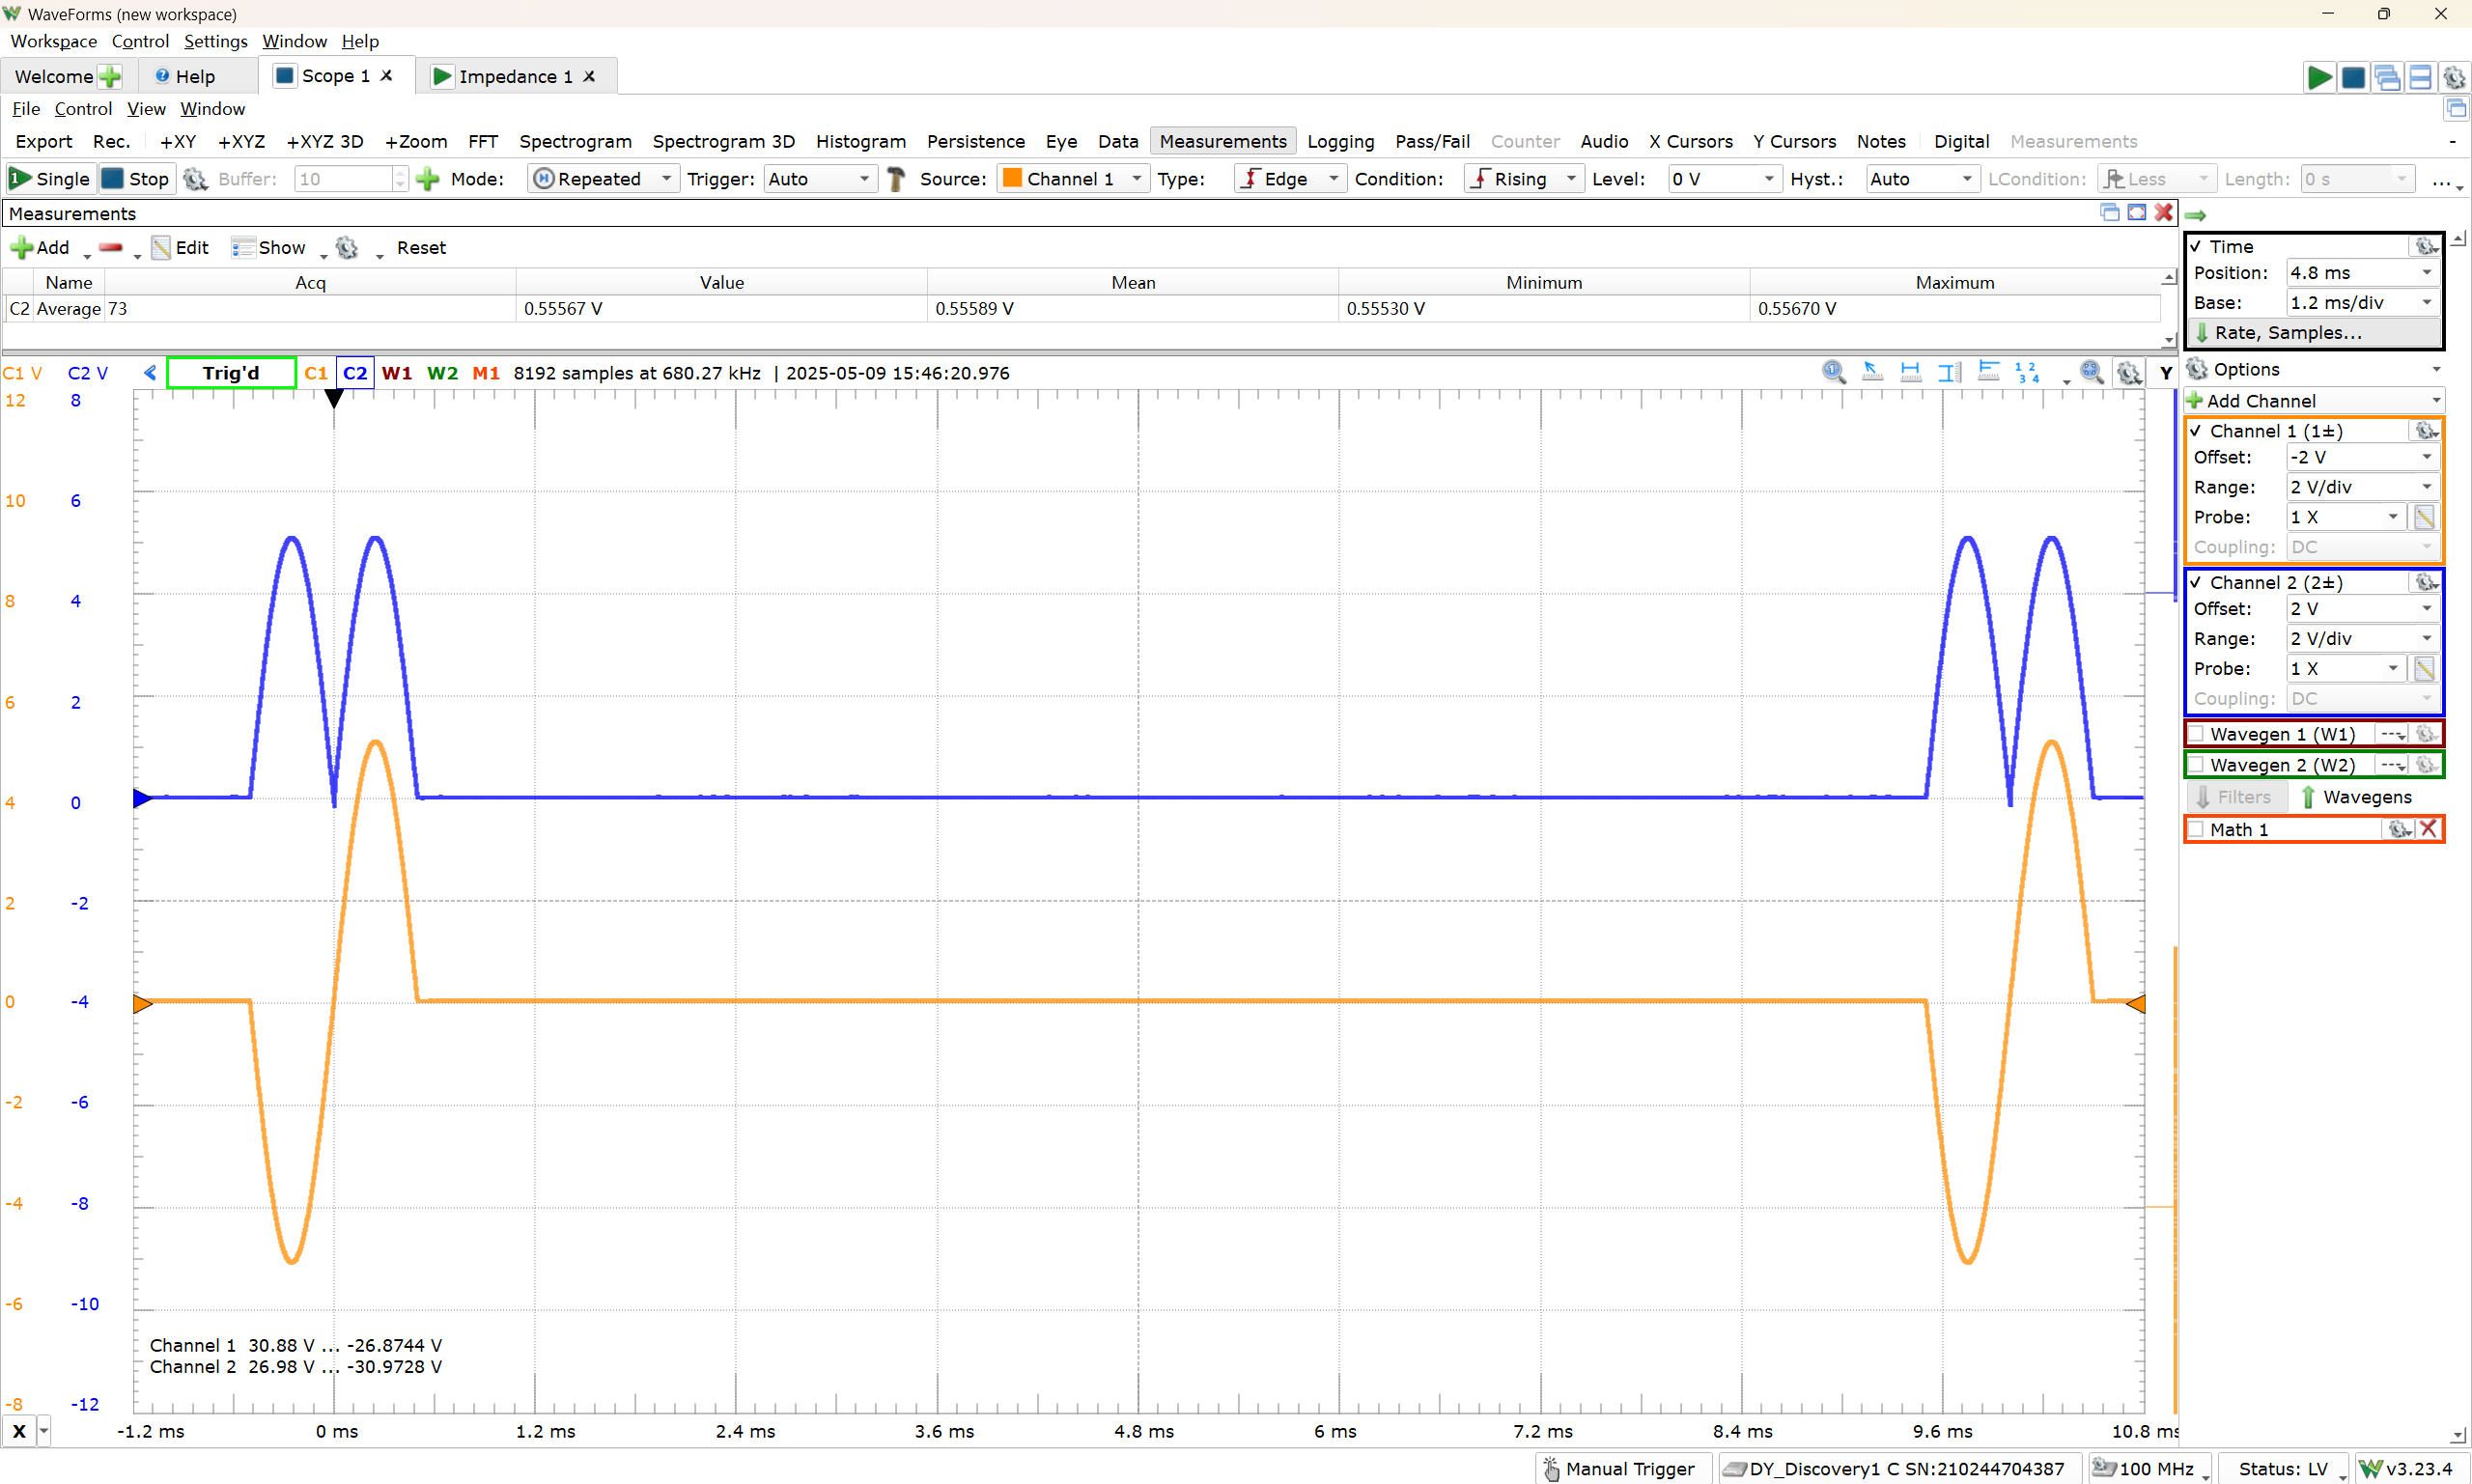
\includegraphics[width=\columnwidth]{LCE-05-精密整流/assets/1N4148/1N4148 brust wave (1 kHz) (2).png}
    \caption{精密整流电路 (diode 1: 1N4148),输入输出波形 (burst input, 5 Vamp @  1 ms / 10 ms),错位显示; CH1 (orange) input, CH2 (blue) output}
\end{figure}

\begin{figure}[H]\centering
    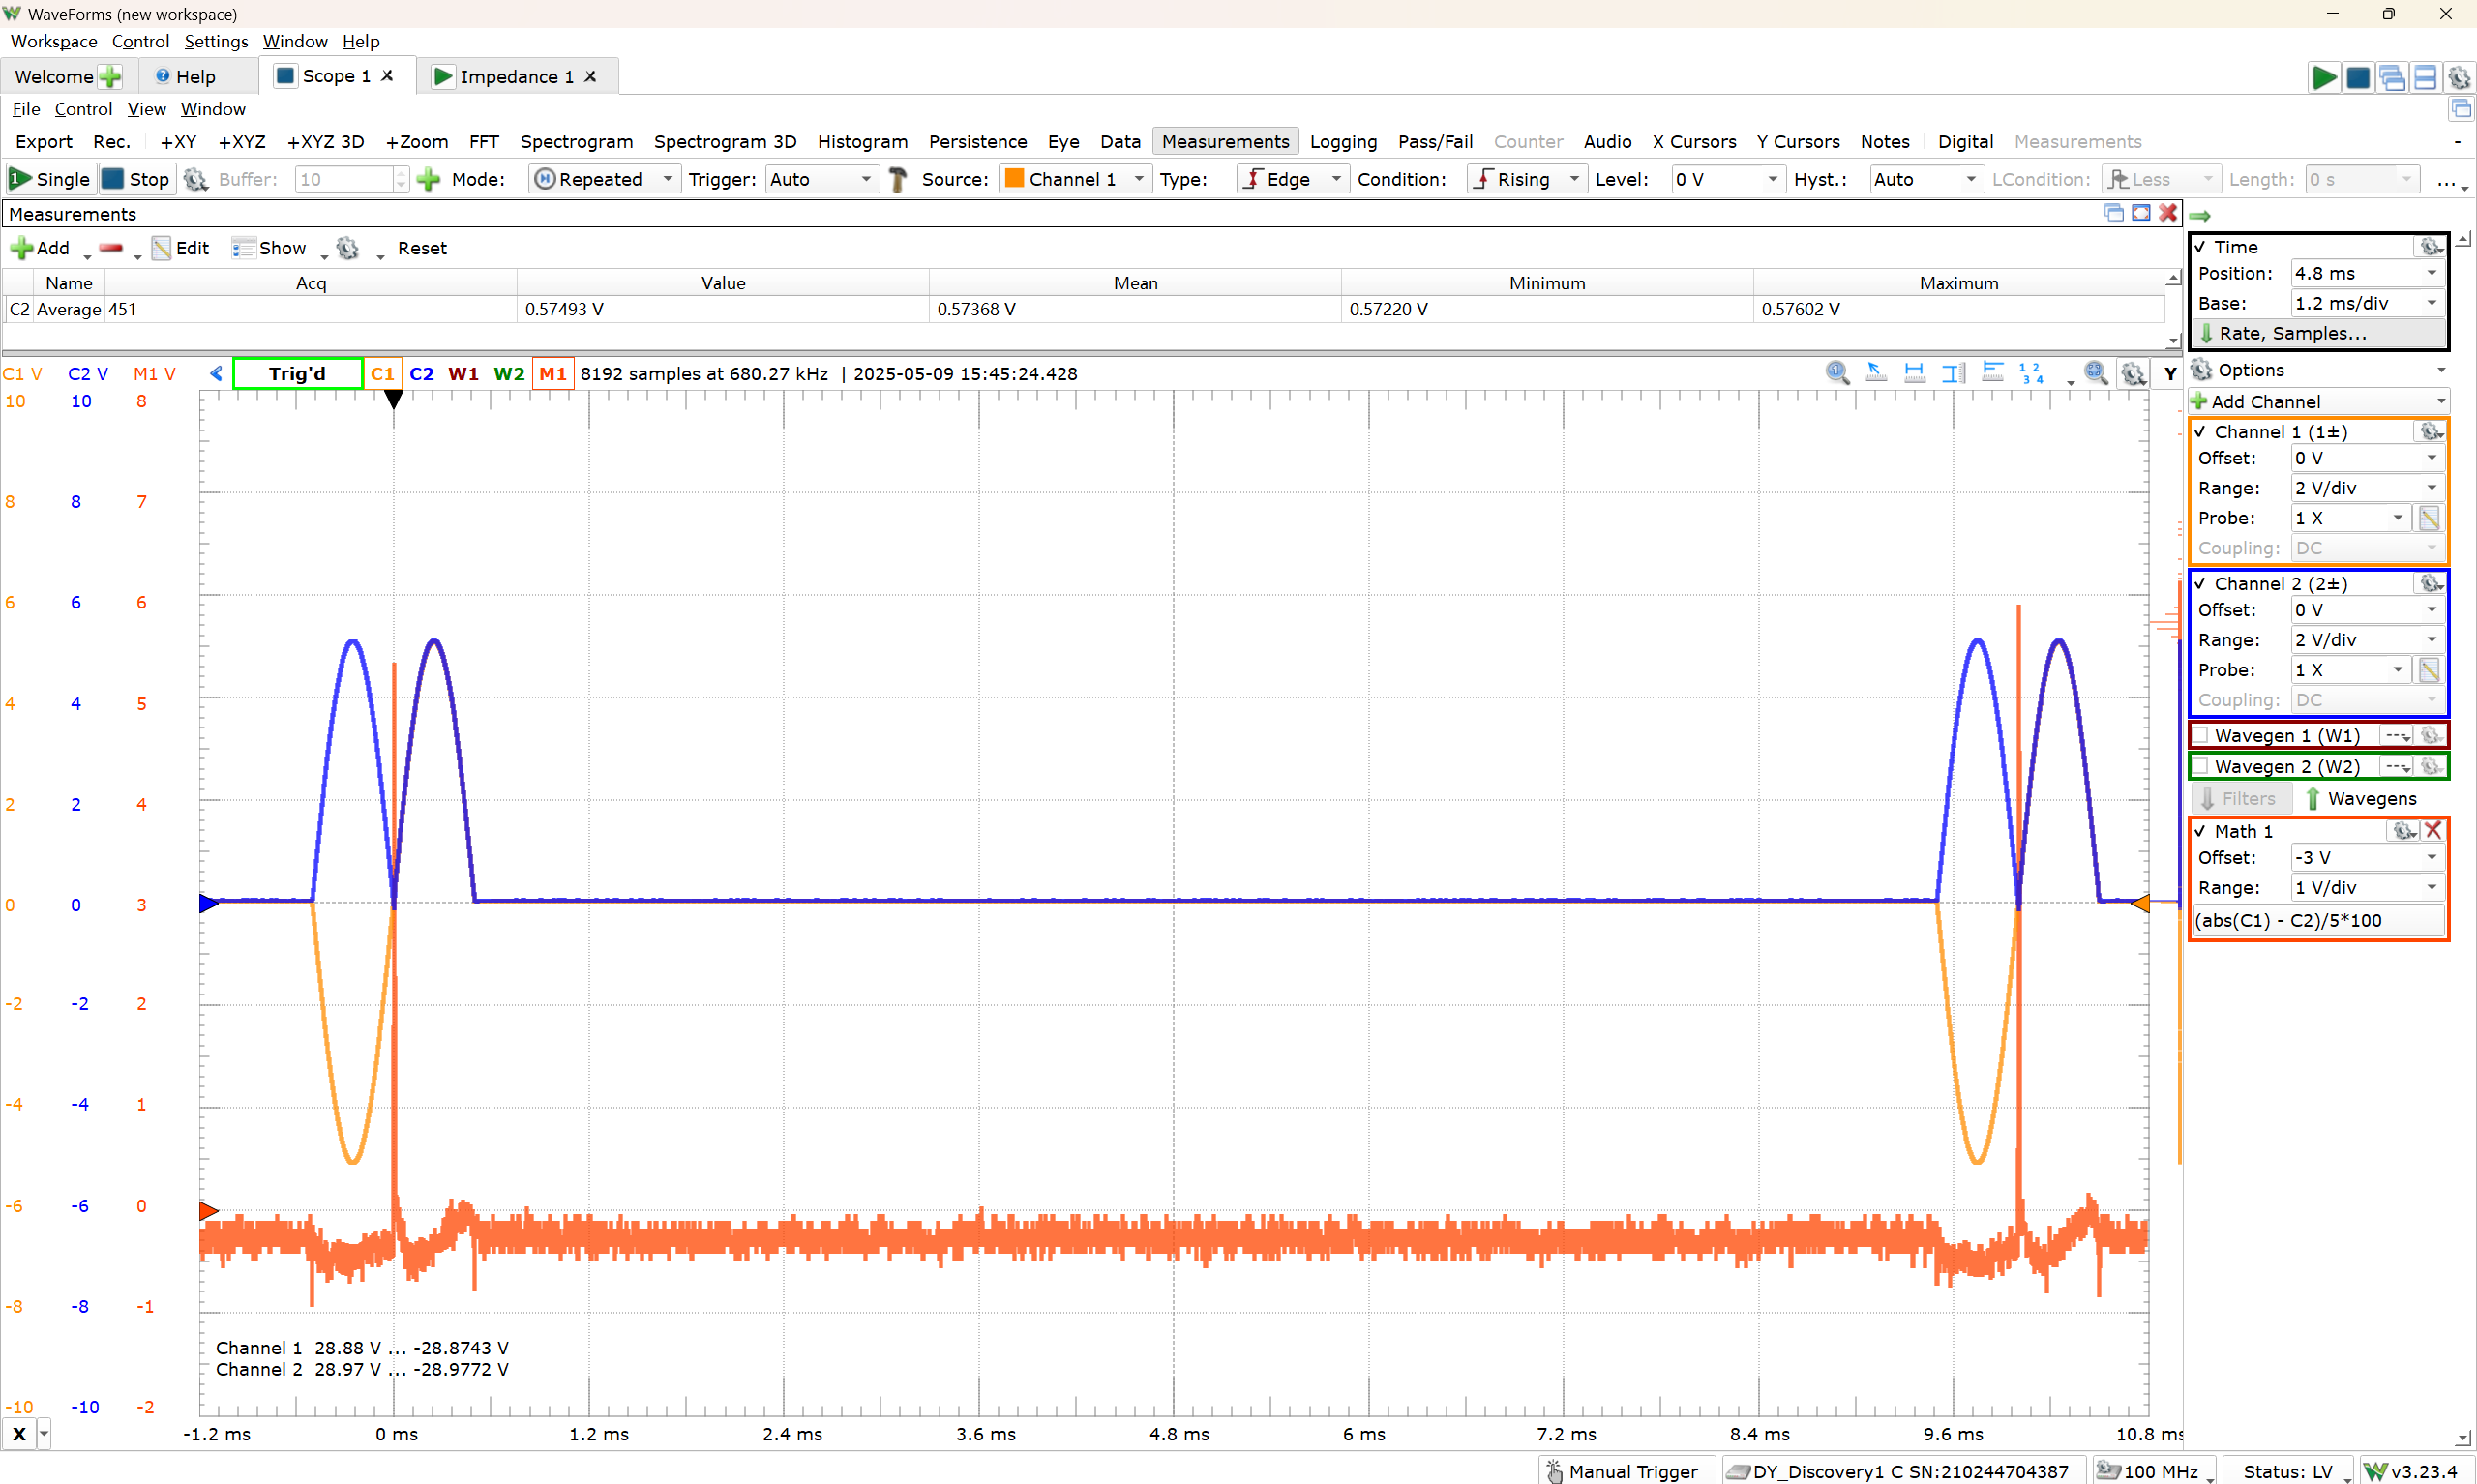
\includegraphics[width=\columnwidth]{LCE-05-精密整流/assets/1N4148/1N4148 brust wave (1 kHz).png}
    \caption{精密整流电路 (diode 1: 1N4148),输入输出波形 (burst input, 5 Vamp @ 1 ms / 10 ms),计算输出平均值和相对误差\\CH1 (orange) input, CH2 (blue) output, M1 (red) relative error}
\end{figure}


\subsection{TI Absolute Circuit (Diode 2, 1N5711)}

将二极管 1N4148 换为 1N5711 (Schottky), 然后重复上面部分实验。

\subsubsection{测量低频输入输出波形}

调整输入信号为 sine wave (5 Vamp @ 50 Hz),得到输入输出波形如下:

\begin{figure}[H]\centering
    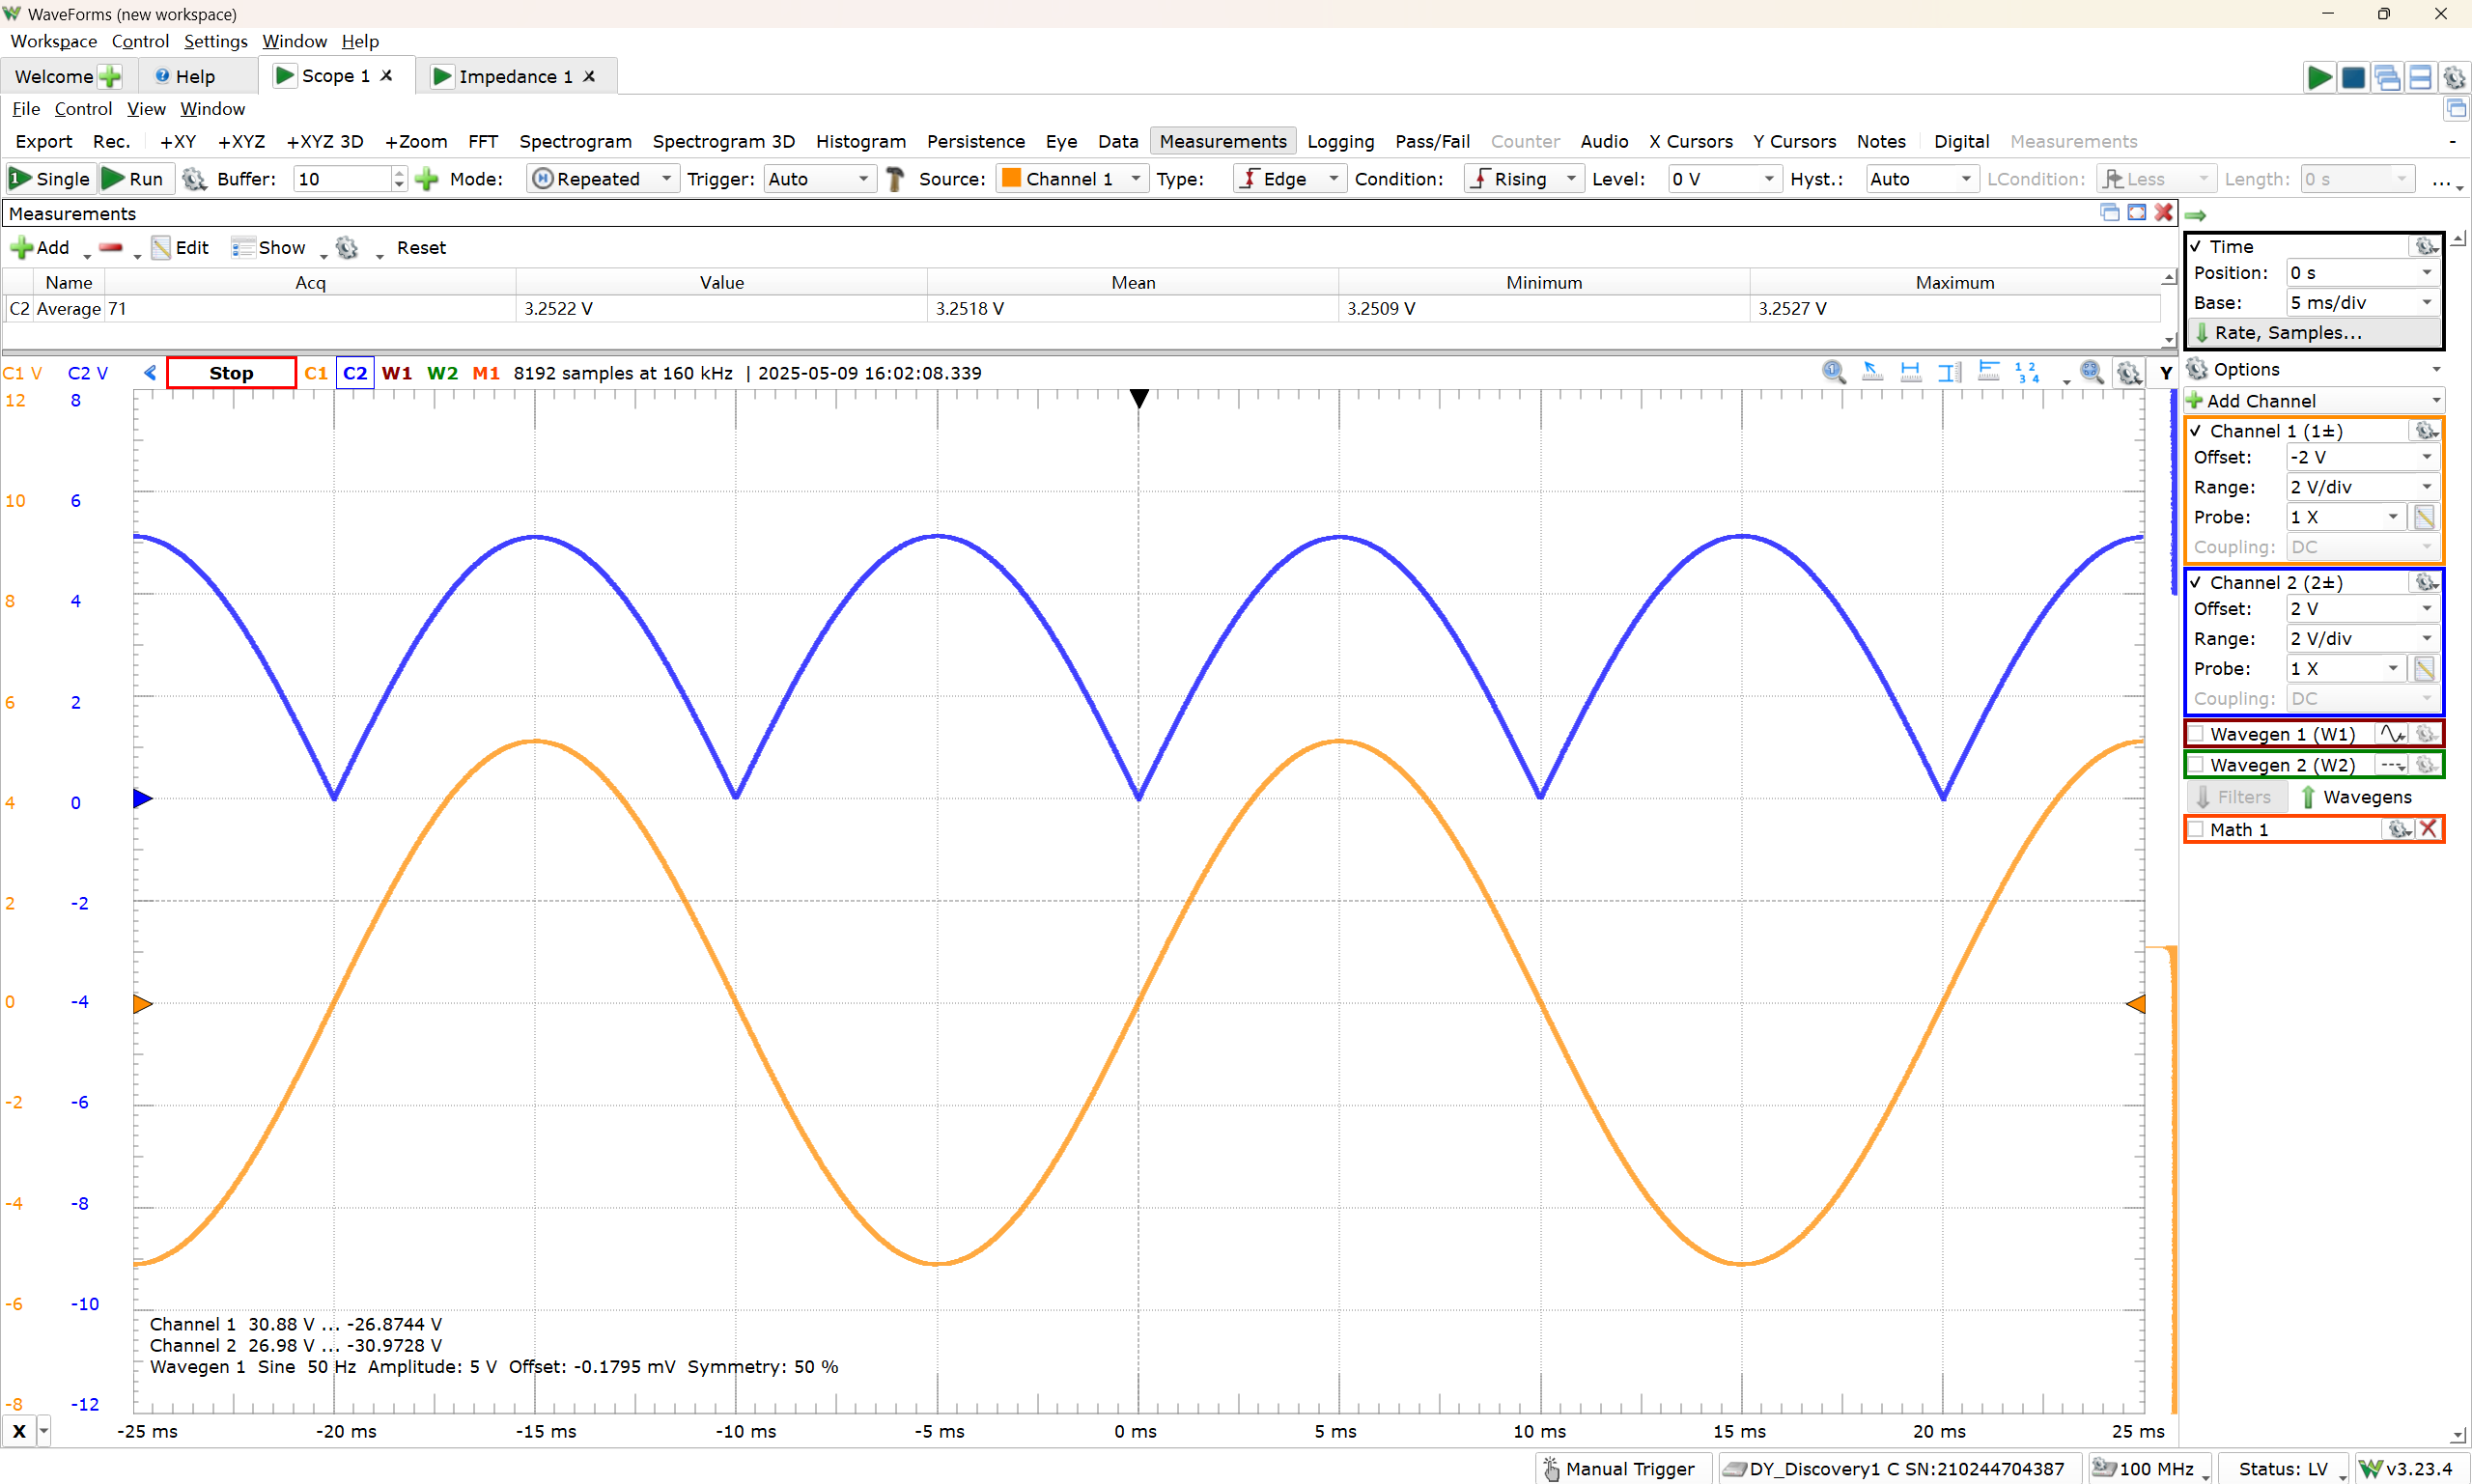
\includegraphics[width=\columnwidth]{LCE-05-精密整流/assets/1N5711/1N5711 input-output waveform (50 Hz) 2.png}
    \vspace*{-7mm}
    \caption{精密整流电路 (diode 2: 1N5711),输入输出波形 (sine input, 5 Vamp @ 50 Hz),错位显示; CH1 (orange) input, CH2 (blue) output}
\end{figure}


\begin{figure}[H]\centering
    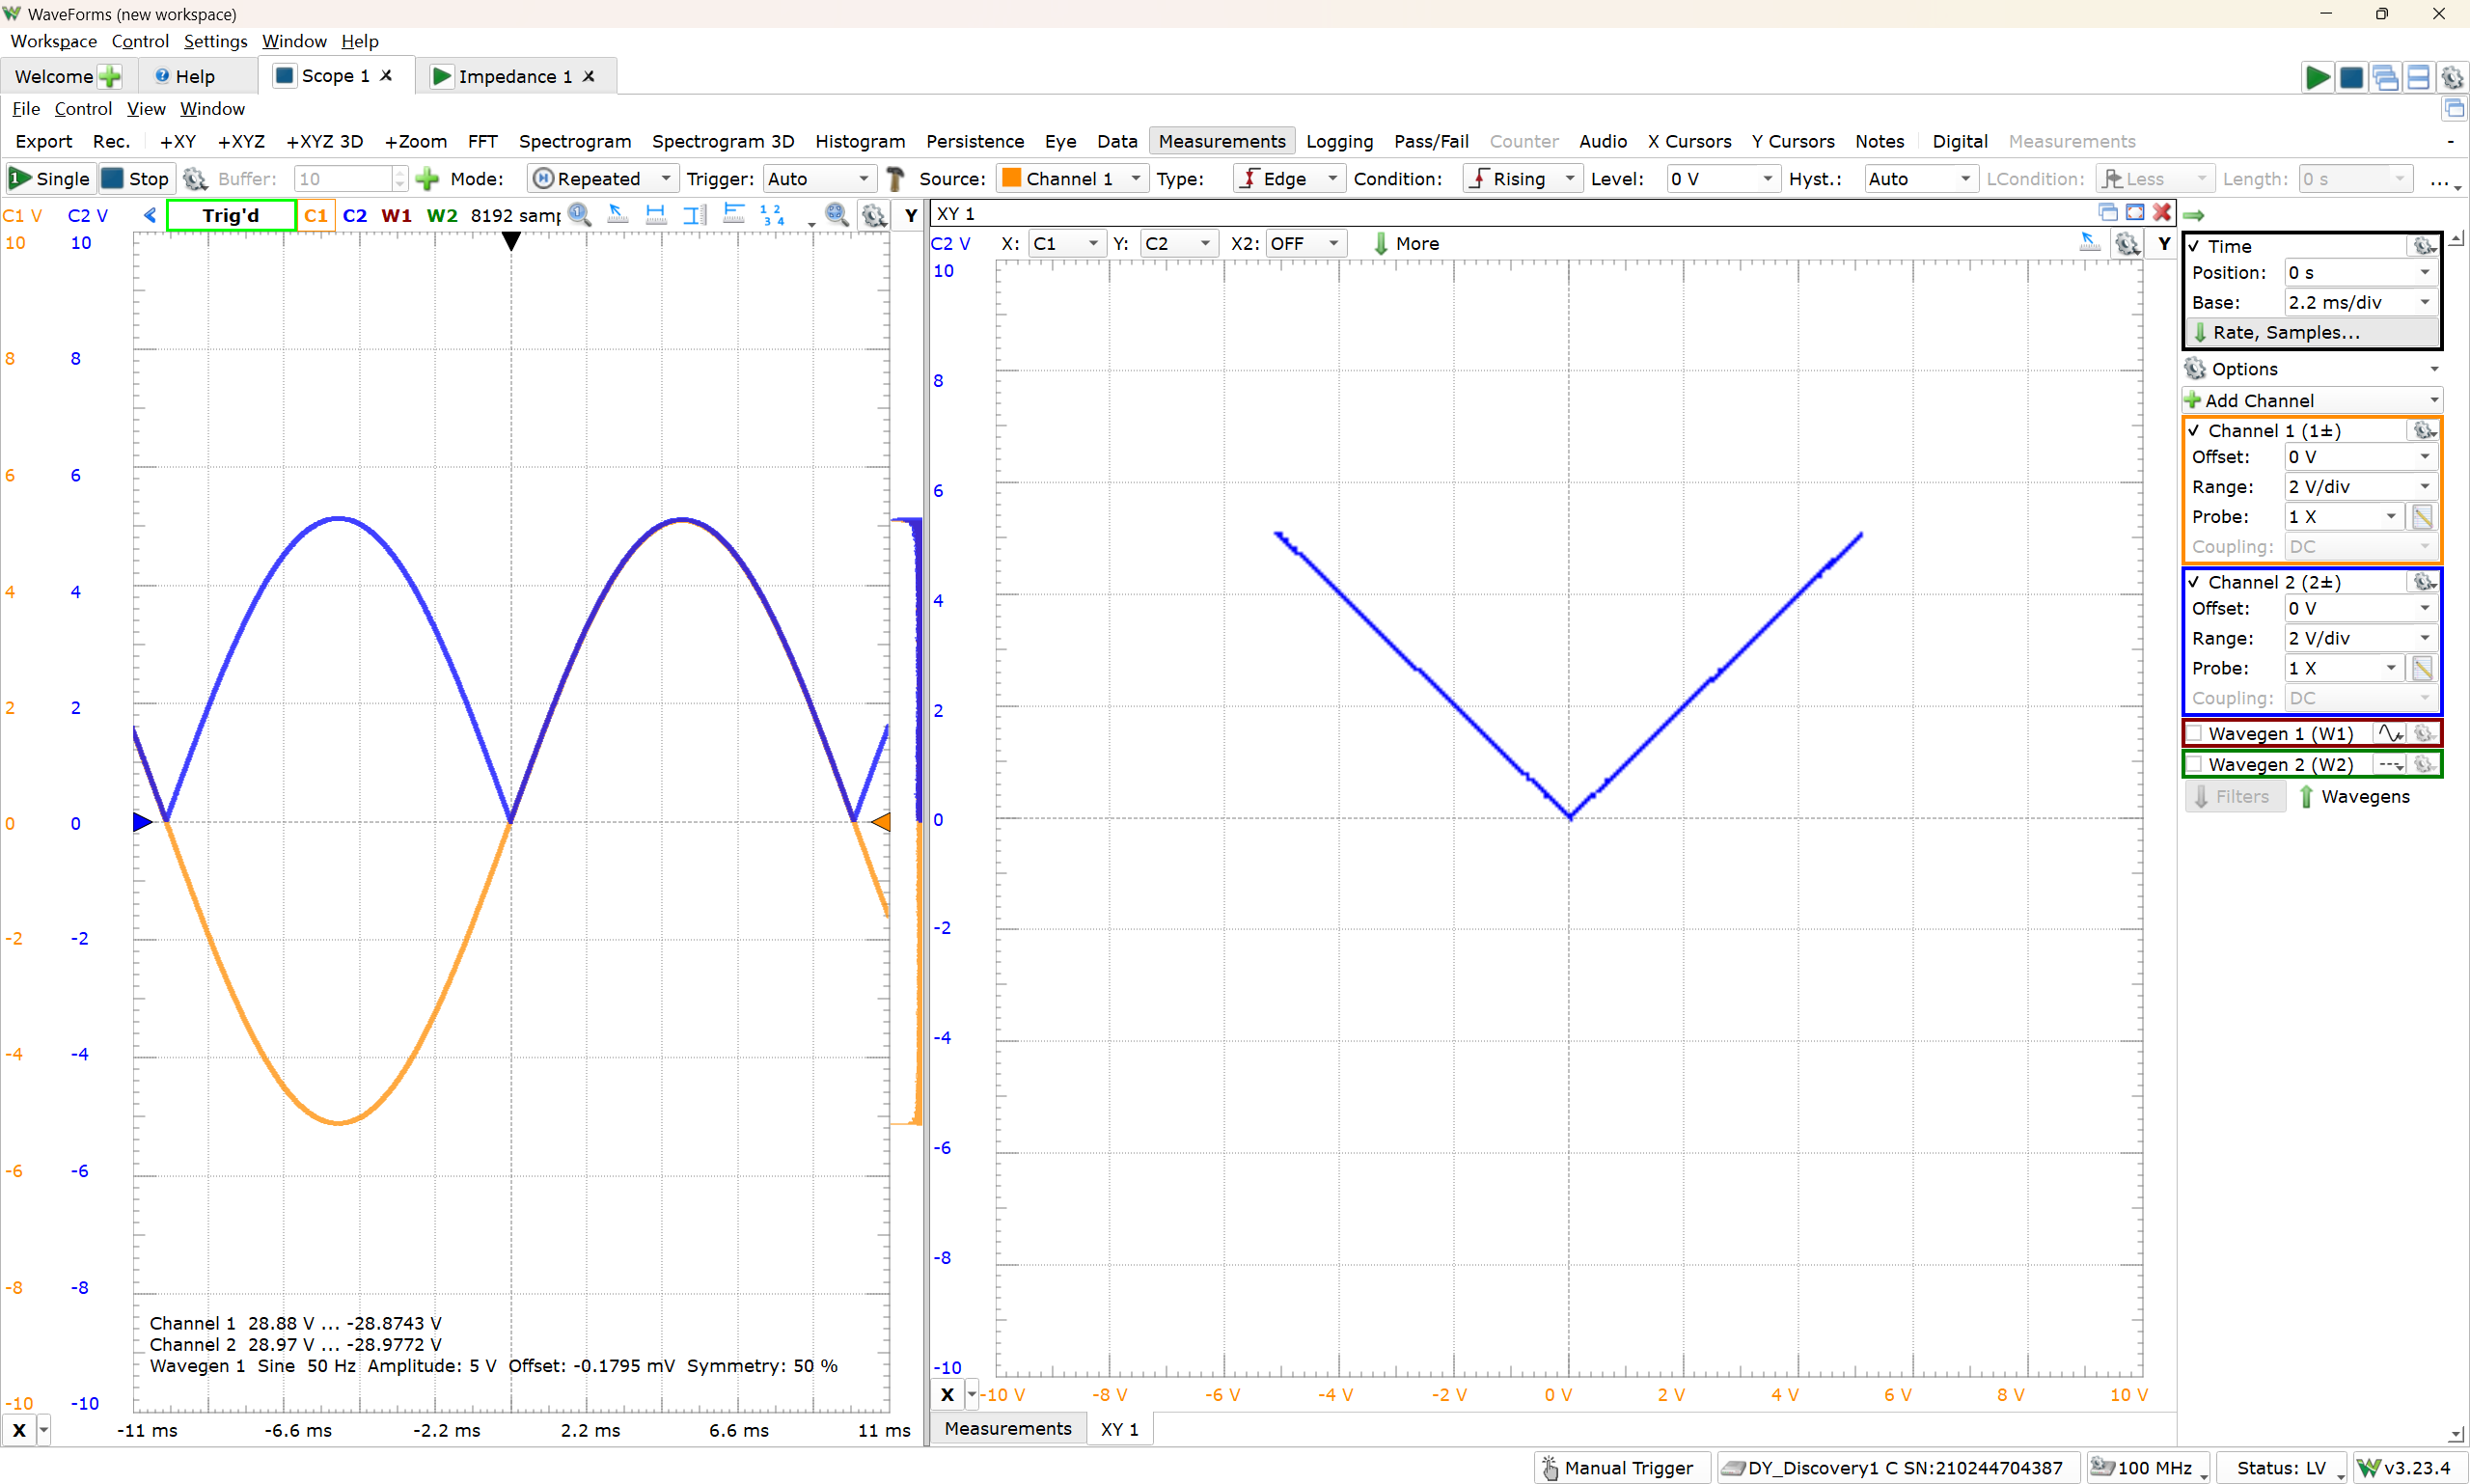
\includegraphics[width=\columnwidth]{LCE-05-精密整流/assets/1N5711/1N5711 input-output waveform (50 Hz) 3.png}
    \vspace*{-7mm}
    \caption{精密整流电路 (diode 2: 1N5711),输入输出波形 (sine input, 5 Vamp @ 50 Hz), X-Y 显示; CH1 (orange) input, CH2 (blue) output}
\end{figure}

\begin{figure}[H]\centering
    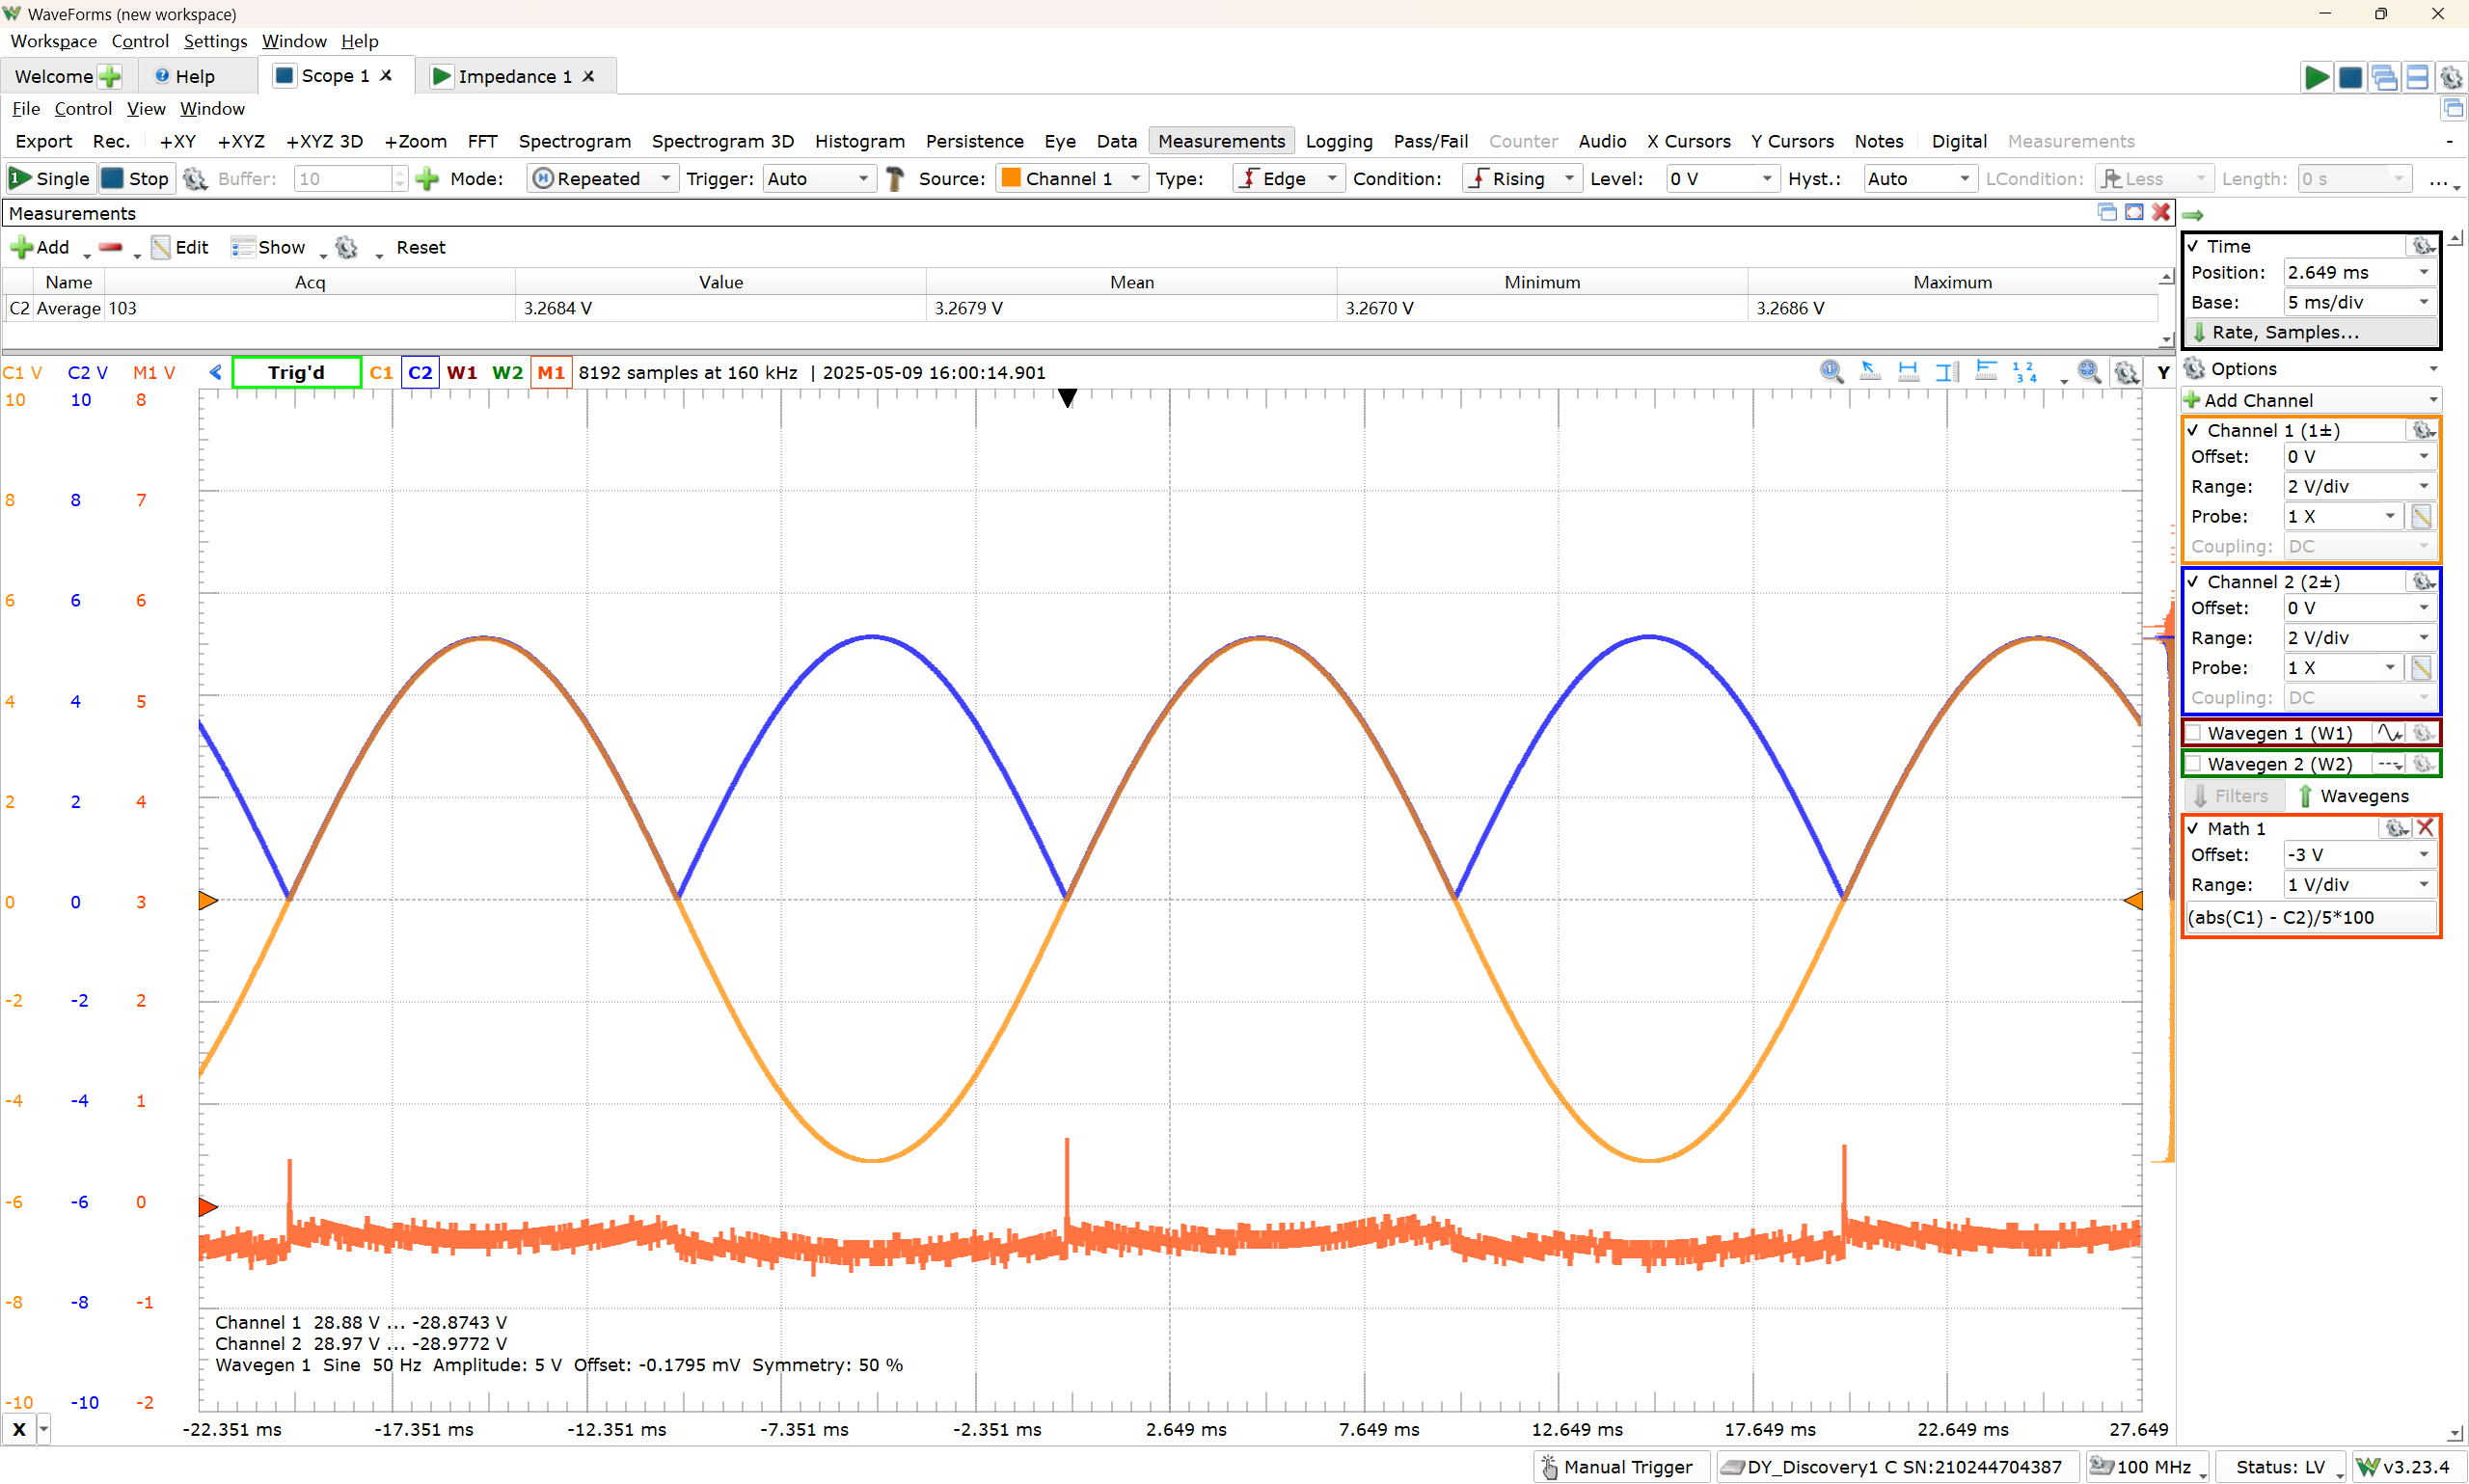
\includegraphics[width=\columnwidth]{LCE-05-精密整流/assets/1N5711/1N5711 input-output waveform (50 Hz) 1.png}
    \vspace*{-9mm}
    \caption{精密整流电路 (diode 2: 1N5711),输入输出波形 (sine input, 5 Vamp @ 50 Hz),计算输出平均值和相对整流误差; CH1 (orange) input, CH2 (blue) output, M1 (red) relative error}
\end{figure}


\subsubsection{测量最高工作频率与频率响应}

类似地,由上一小节我们得到 $(V_{out})_{mean}^{\mathrm{50 Hz}} = 3.2679 \ \mathrm{V}$,则最高工作频率处有 $(V_{out})_{mean}^{f_{max}} = 3.2352 \ \mathrm{V}$。调整输入频率,得到结果如下:

\begin{figure}[H]\centering
    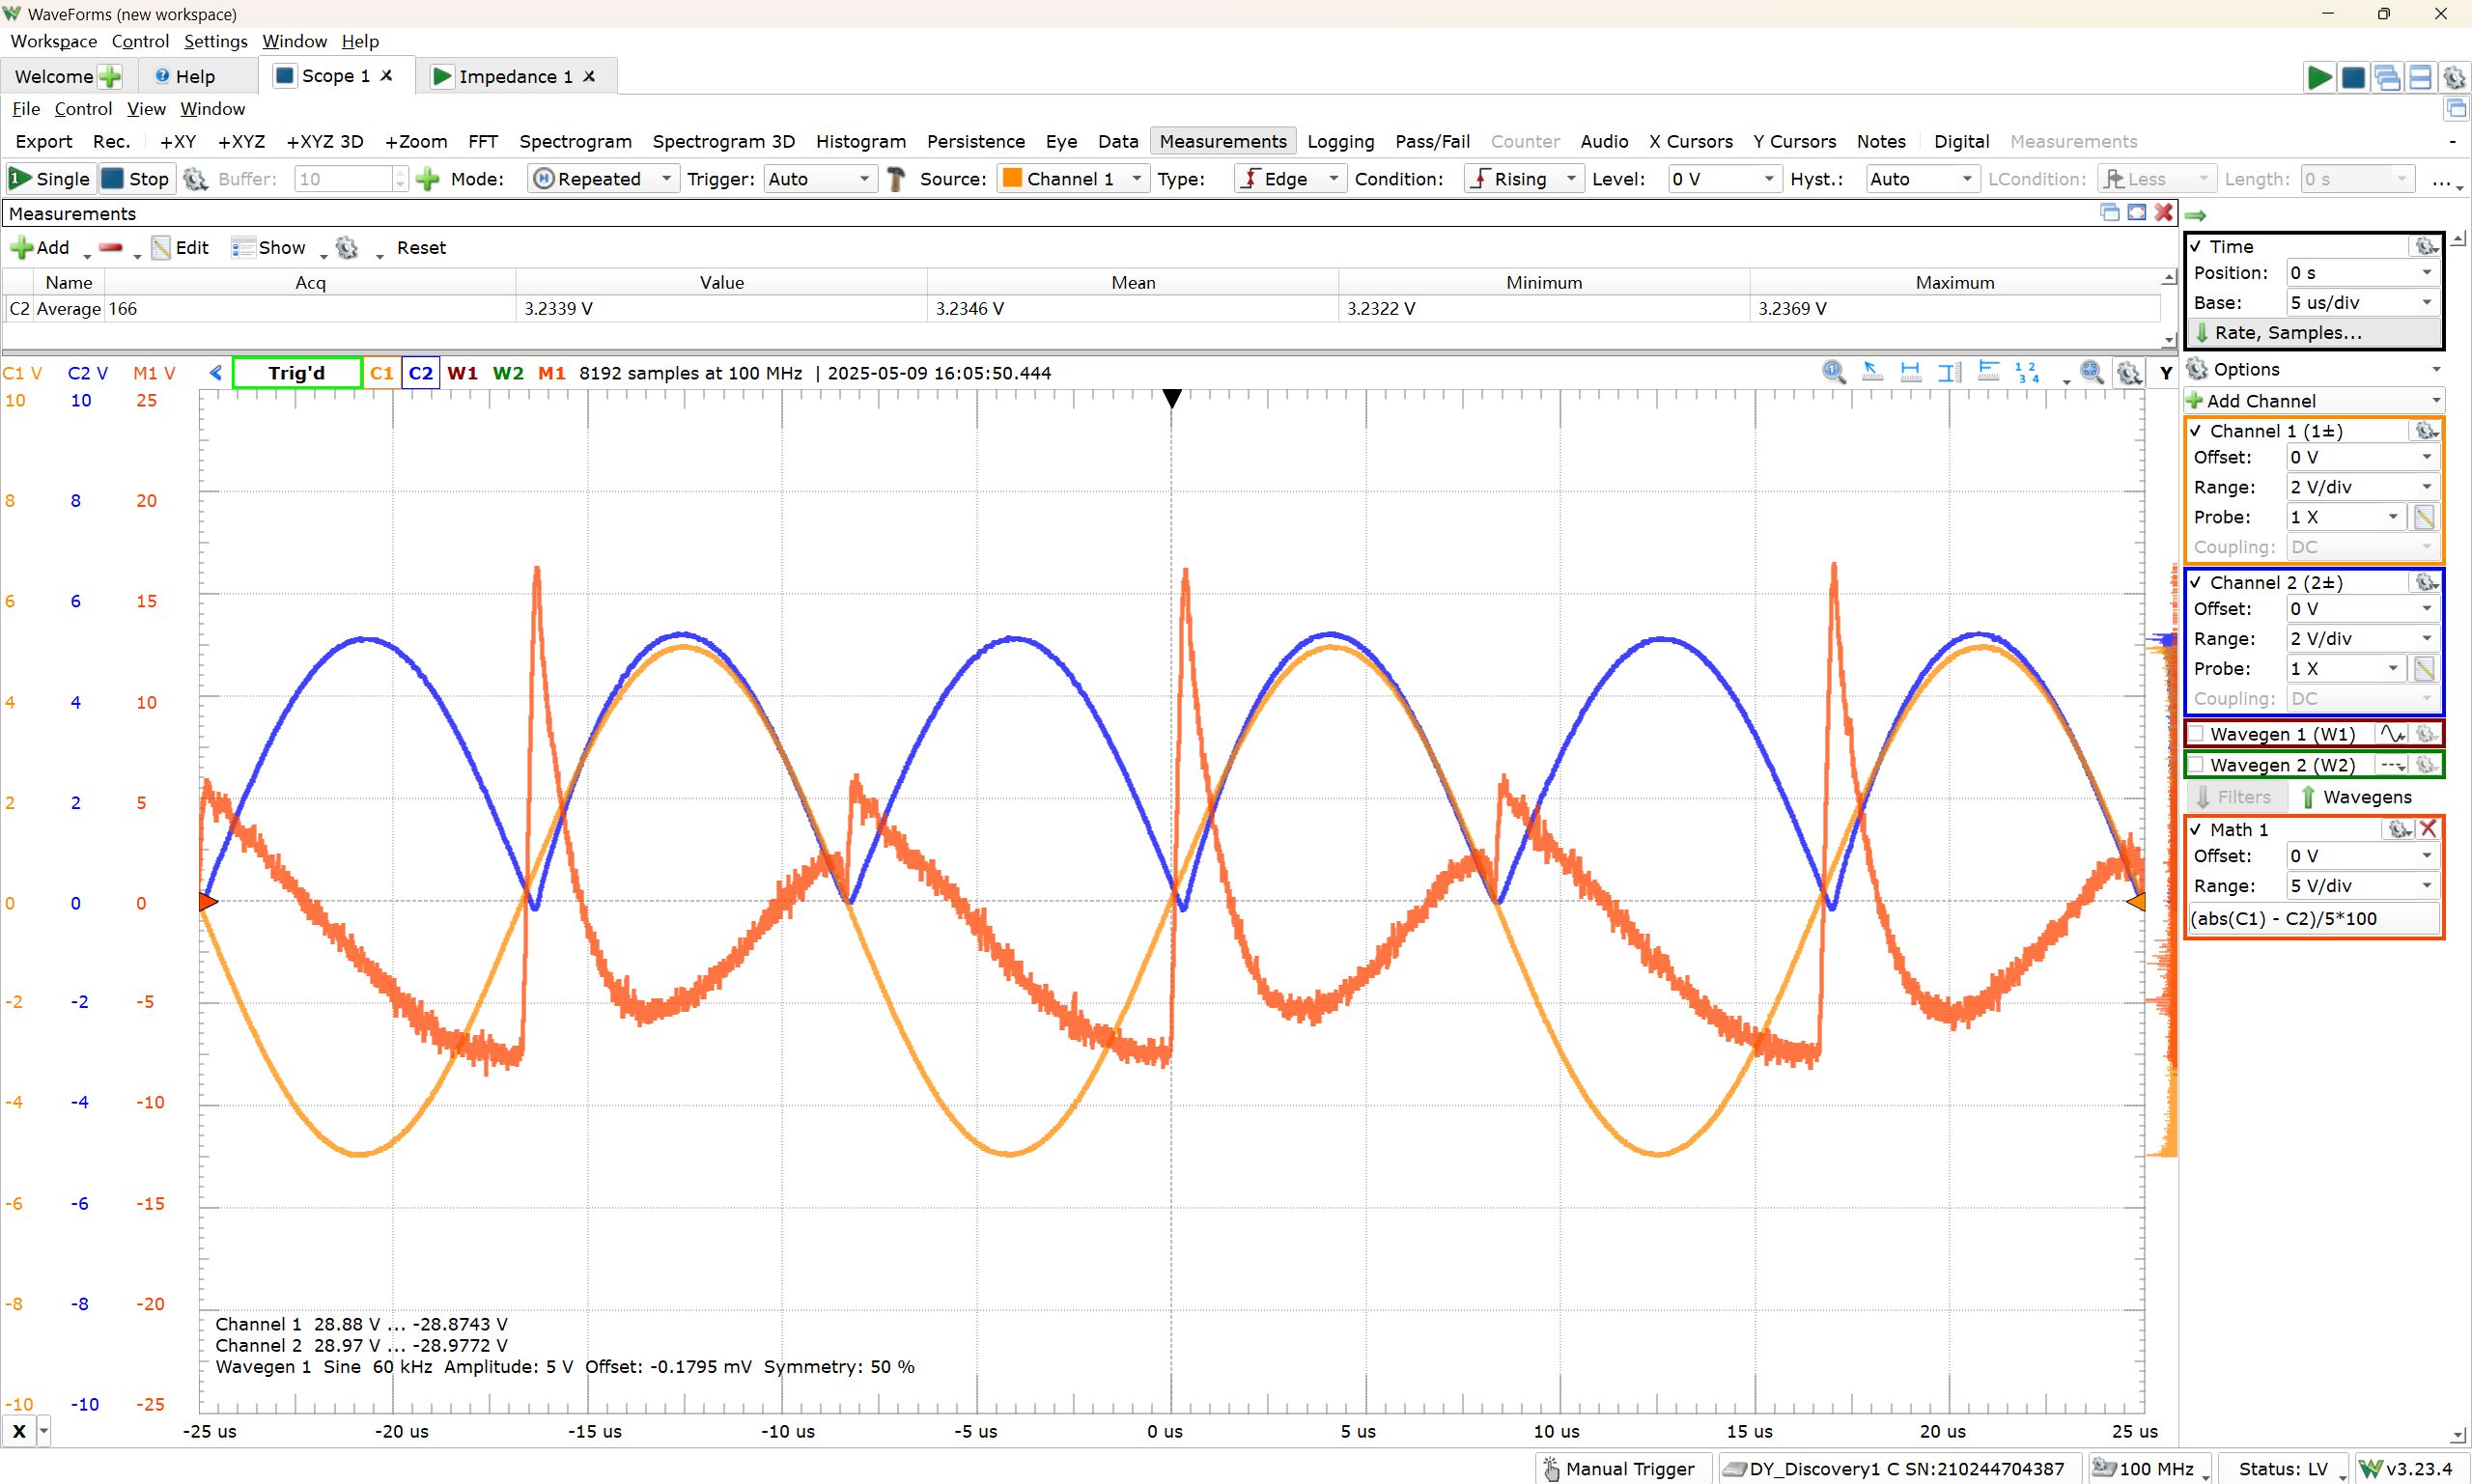
\includegraphics[width=\columnwidth]{LCE-05-精密整流/assets/1N5711/1N5711 input-output waveform (max 70 kHz) with error and mean.png}
    \vspace*{-9mm}
    \caption{精密整流电路 (diode 2: 1N5711),最高工作频率 (sine input, 5 Vamp),$f = 60 \ \mathrm{kHz}$, $(V_{out})_{mean} = 3.2346 \ \mathrm{V}$; CH1 (orange) input, CH2 (blue) output, M1 (red) relative error}
\end{figure}


\section{思考题}

\subsection{计算输入 50 Hz 时,输出信号中 100 Hz 分量的幅度值,以及输出通过滤波器后的幅度值}

对于精密整流电路 (diode 2: 1N5711),我们导出输入信号为 sine wave (5 Vamp @ 50 Hz) 时的输出,并对输出信号作 FFT (Fast Fourier Transform) 以计算 100 Hz 分量的幅度值。结果如下:

\begin{figure}[H]\centering
    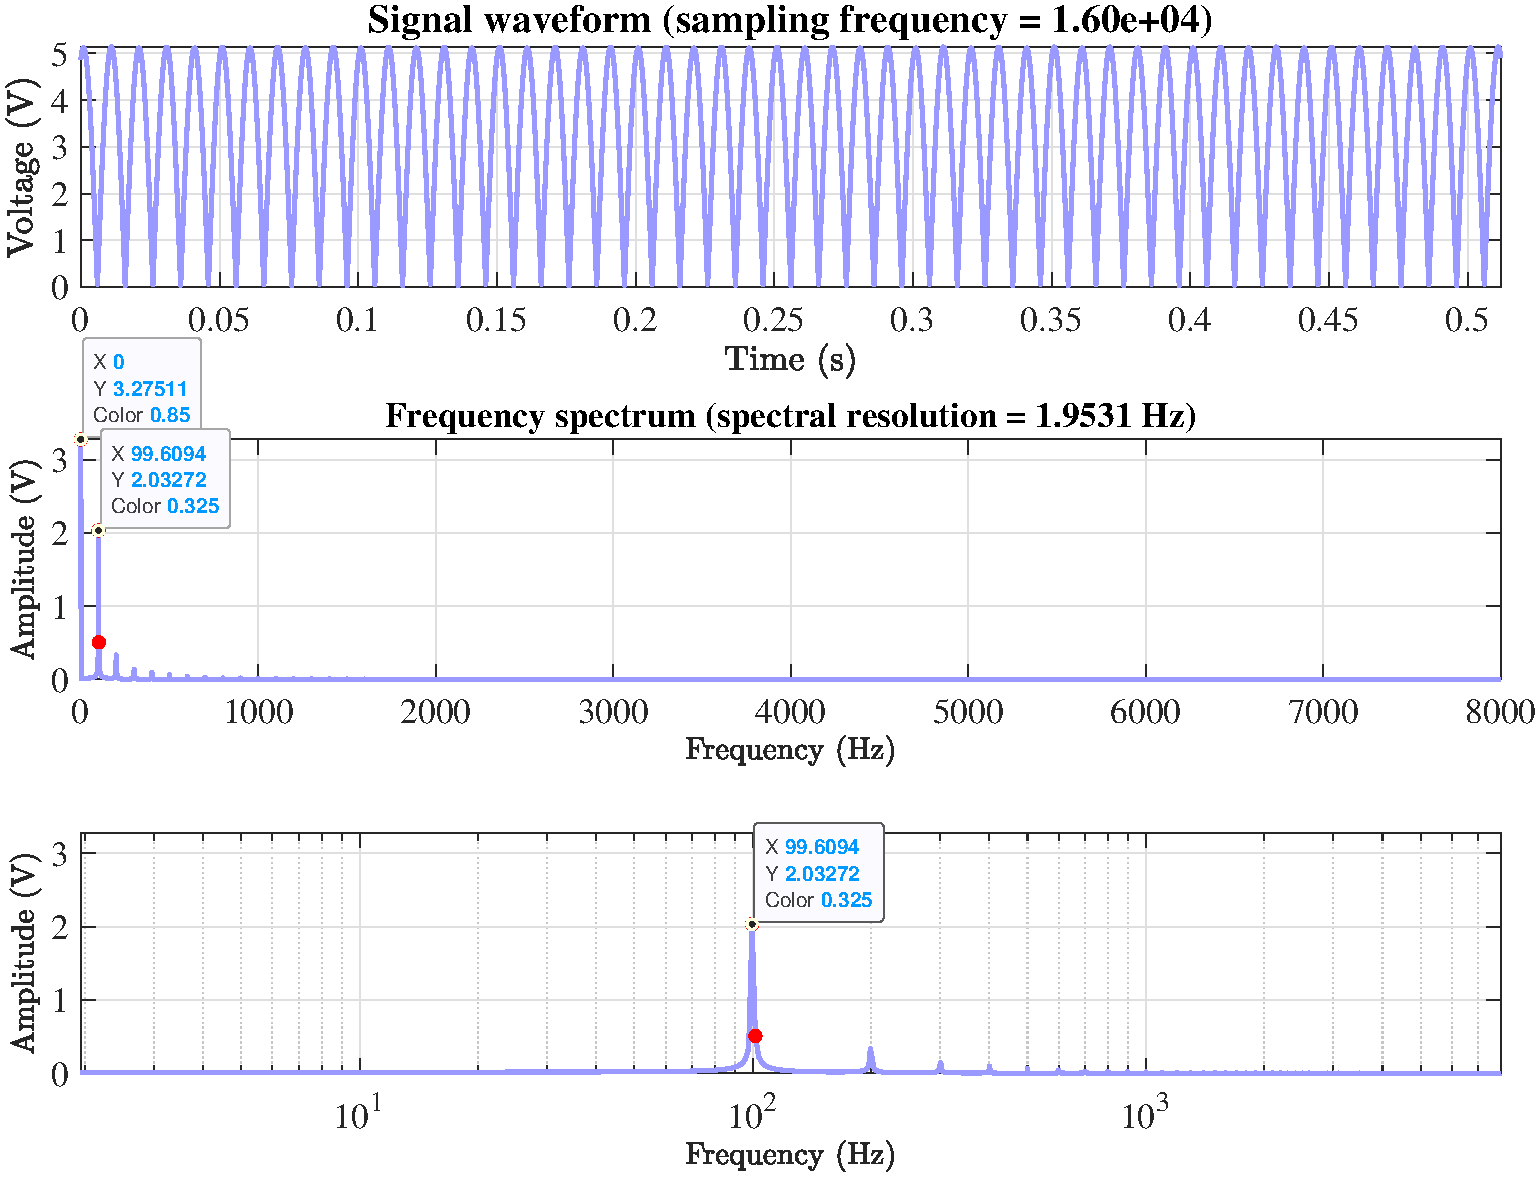
\includegraphics[width=\columnwidth]{LCE-05-精密整流/assets/1N5711/FFT.pdf}
    \caption{精密整流电路 (diode 2: 1N5711), FFT result of the output signal (sine input, 5 Vamp @ 50 Hz)}
\end{figure}

由图中读出 100 Hz 分量的幅度值,以及输出分别通过理想二阶、三阶滤波器后的幅度值 ($f_c = 10 \ \mathrm{Hz}$) 为:
\begin{gather}
(V_{100 \ \mathrm{Hz}})_{amp} = 2.03272 \ \mathrm{V},\quad 
(V_{100 \ \mathrm{Hz}})_{amp}^{\text{2-order\ LPH}} = 20.3272 \ \mathrm{mV},\quad
(V_{100 \ \mathrm{Hz}})_{amp}^{\text{3-order\ LPH}} = 2.03272 \ \mathrm{mV}
\end{gather}

\subsection{精密整流电路对运放及二极管有何要求?}

\begin{enumerate}
\item 对运放:需要高增益、高输入阻抗且高 SR 运放,减小电路对输入影响的同时,获得较稳定的输出与较好的带宽;另外,高速、低温漂、低噪声、高 CMRR 和 高 PSRR 能够进一步提升电路性能;如果需要在低电源电压中工作,运放最好是 rail-to-rail 运放。

\item 对二极管:选用结电容小、开关速度快的二极管,以此提高电路的最高工作频率;同时,反向漏电流不宜过大,以免影响二极管断开时的输出精度。
\end{enumerate}



\subsection{输入更改为 51 Hz, 52 Hz 后,万用表 RMS 挡读数明显抖动,试分析原因}

万用表的 AD 转换一般是双积分型,会对分别对输入电压和参考电压进行共两次积分。为抑制工频干扰,积分的时间常数常选用 0.2 s (1 / 50 Hz) 或其倍数。当输入频率为 51 Hz, 52 Hz 时,信号周期与积分周期存在偏差,不同的积分起点会得到不同的积分结果,导致最终示数出现明显抖动。

% \subsection*{4.1 \ \ }
% \subsection*{4.2 \ \ }
% \subsection*{4.3 \ \ }
% \subsection*{4.4 \ \ }
% \subsection*{4.5 \ \ }
% \subsection*{4.6 \ \ }


\section{运放设计预告}

% 这里是链接
See \href{https://yidingg.github.io/YiDingg/\#/ElectronicDesigns/Basic\%20Two-Stage\%20Op\%20Amp\%20using\%20Discrete\%20MOSFETs
}{ % 这里是文字
Basic Two-Stage Op Amp using Discrete MOSFETs {\color{black}\footnotesize (https://yidingg.github.io/YiDingg/\#/ElectronicDesigns/Basic\%20Two-Stage\%20Op\%20Amp\%20using\%20Discrete\%20MOSFETs)}
} 
and 
% 这里是链接
\href{https://yidingg.github.io/YiDingg/\#/ElectronicDesigns/\%CE\%BCA741\%20using\%20Discrete\%20BJTs\%20(SOT-23)
}{ % 这里是文字
μA741 (Op Amp) using Discrete BJTs (SOT-23) \\ {\color{black}\footnotesize (https://yidingg.github.io/YiDingg/\#/ElectronicDesigns/\%CE\%BCA741\%20using\%20Discrete\%20BJTs\%20(SOT-23))}
}
for more details.

\begin{figure}[H]\centering
\begin{subfigure}[b]{0.5\columnwidth}\centering
    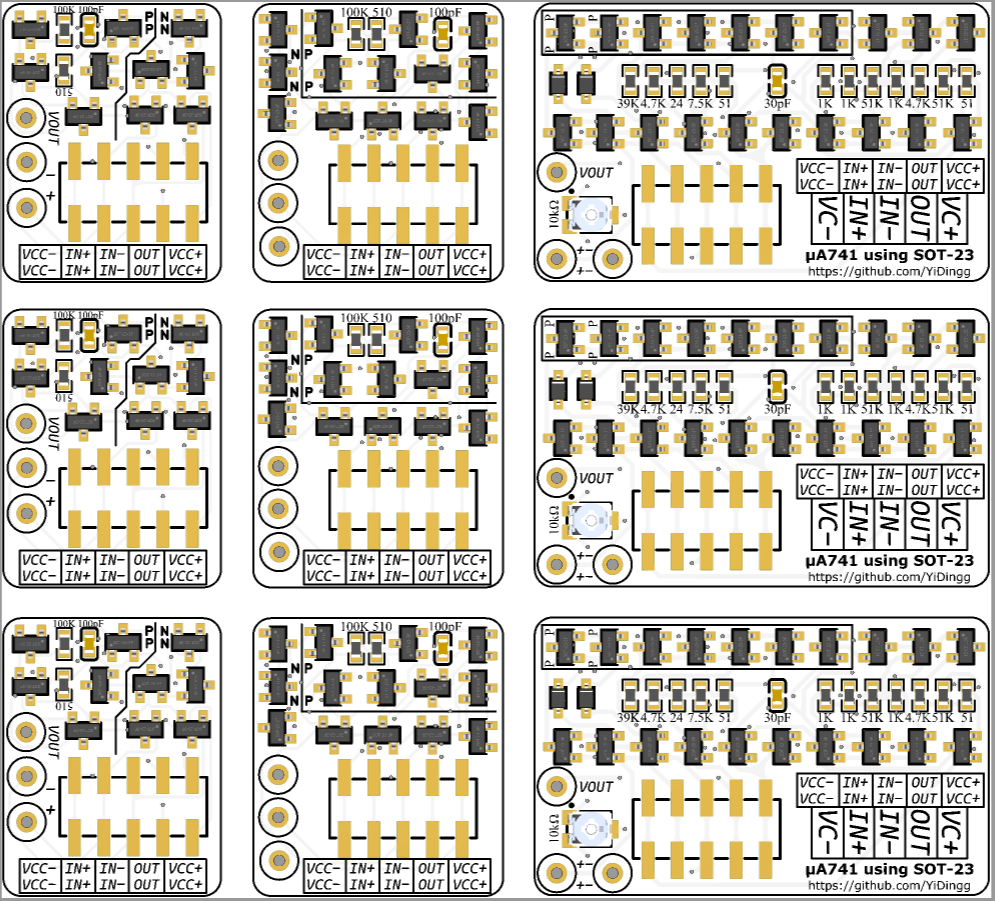
\includegraphics[height=200pt]{LCE-05-精密整流/preview/assets/op amp 1.png}
    \caption{Top view}
\end{subfigure}\hfill
\begin{subfigure}[b]{0.5\columnwidth}\centering
    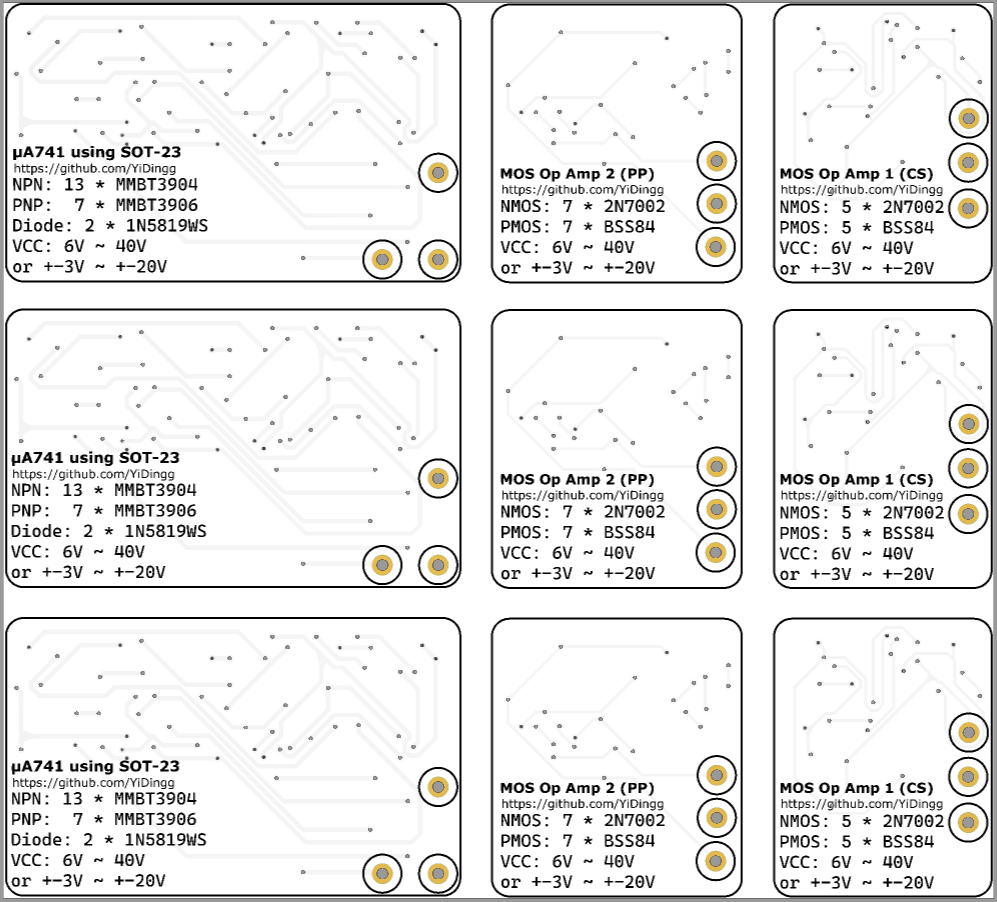
\includegraphics[height=200pt]{LCE-05-精密整流/preview/assets/op amp 2.png}
    \caption{Bottom view}
\end{subfigure}
\caption{Basic two-stage CMOS op amps and uA741 using discrete transistors (package SOT-23)}
\end{figure}















































\newpage
% 附录 A
\newpage
\vspace*{\fill}\begin{center}\Huge{\bfseries 
    附录 A\hspace*{20pt} 预习报告
}\end{center}\addcontentsline{toc}{section}{附录 A\hspace*{6pt} 预习报告} 
\begin{figure}[H]\centering
    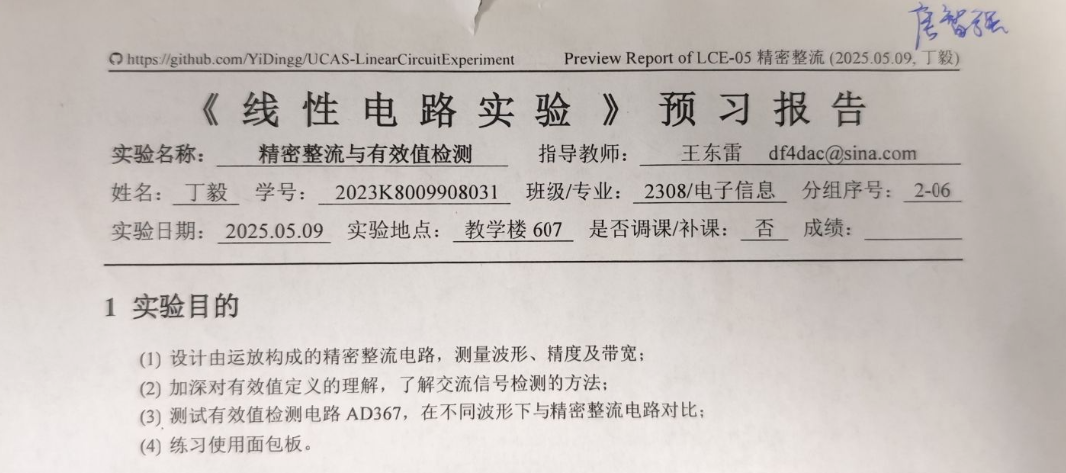
\includegraphics[width=\columnwidth]{LCE-05-精密整流/assets/appendix/image.png}
\end{figure}
\vspace*{\fill}
\thispagestyle{fancy} 
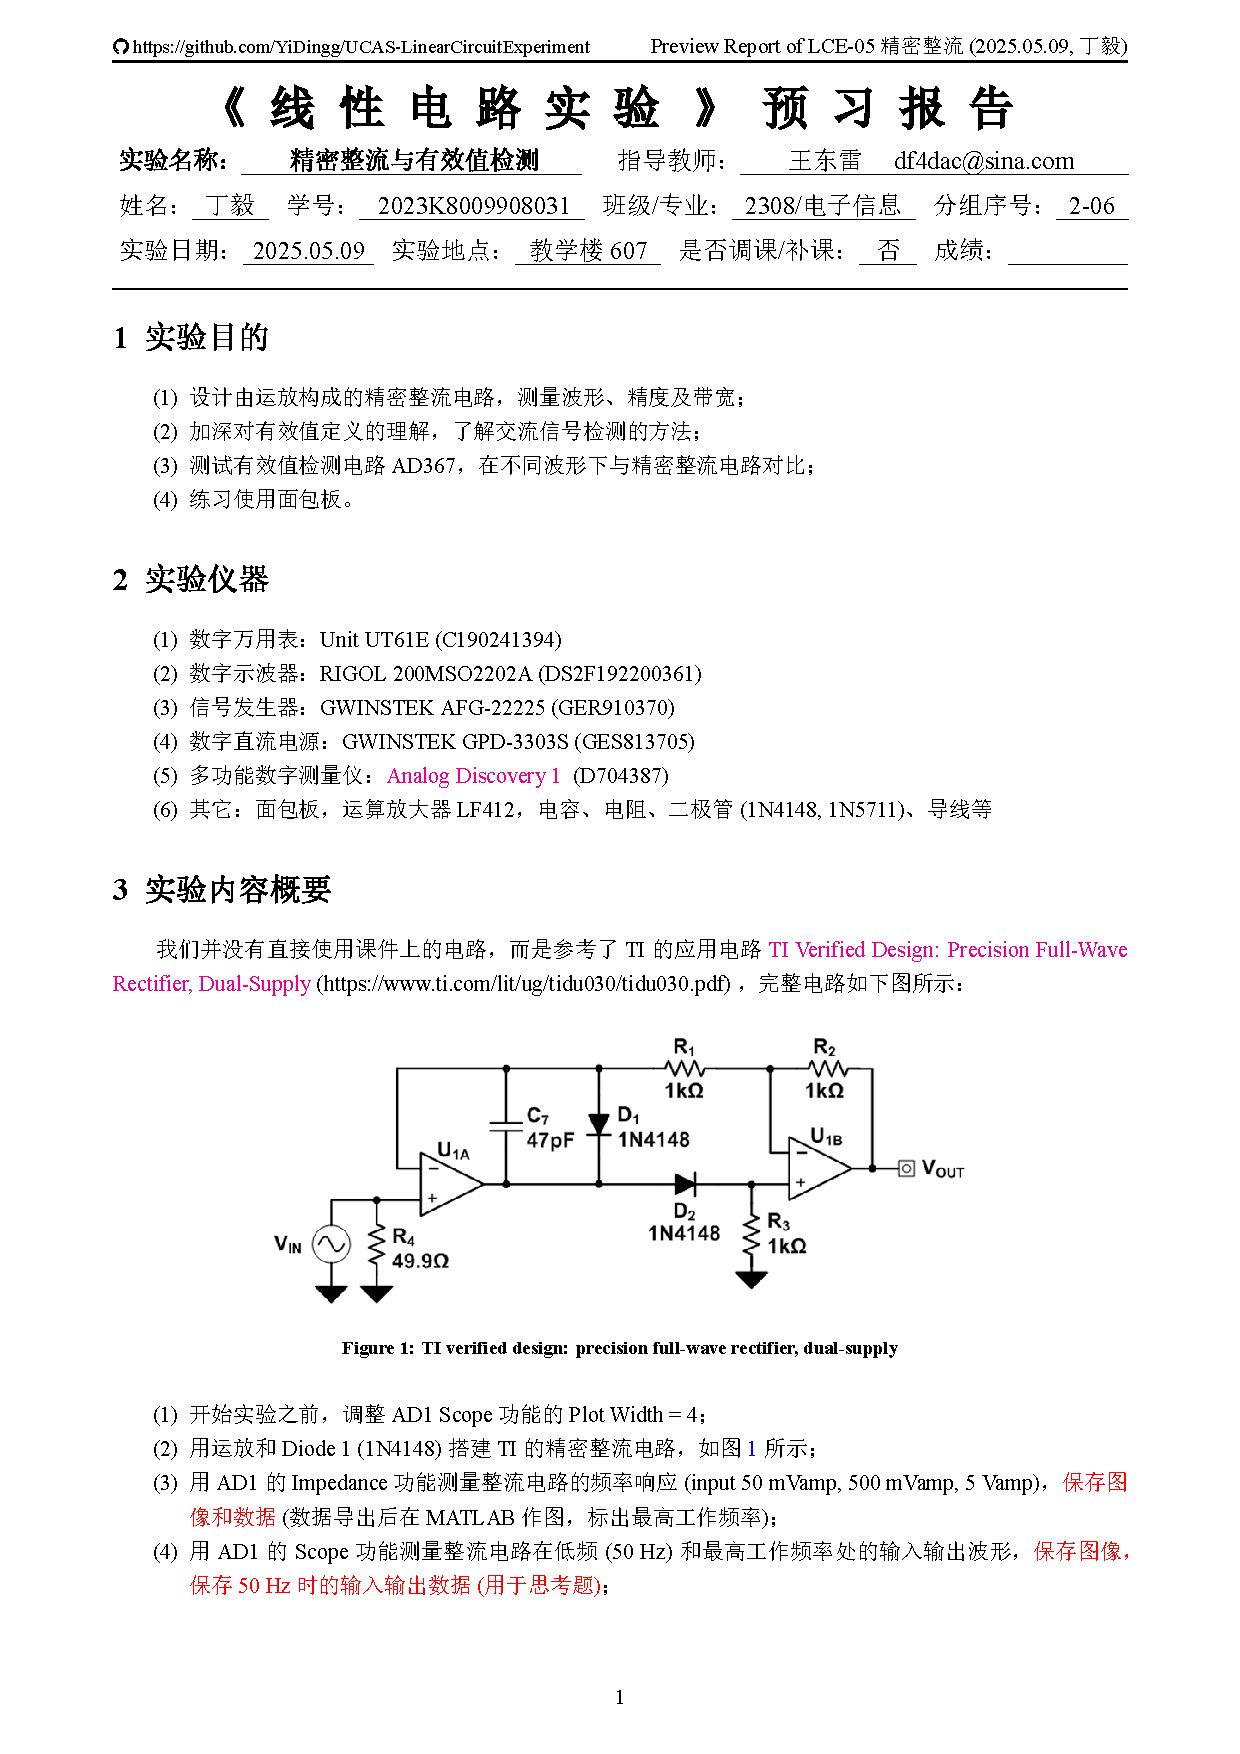
\includepdf[pages={-}]{LCE-05-精密整流/preview/LCE-05 (preview report).pdf}



% 附录 B
\section*{附录 B\hspace*{20pt} 原始数据记录表}
\addcontentsline{toc}{section}{附录 B\hspace*{6pt} 原始数据记录表} 
\thispagestyle{fancy} 
\begin{figure}[H]\centering
    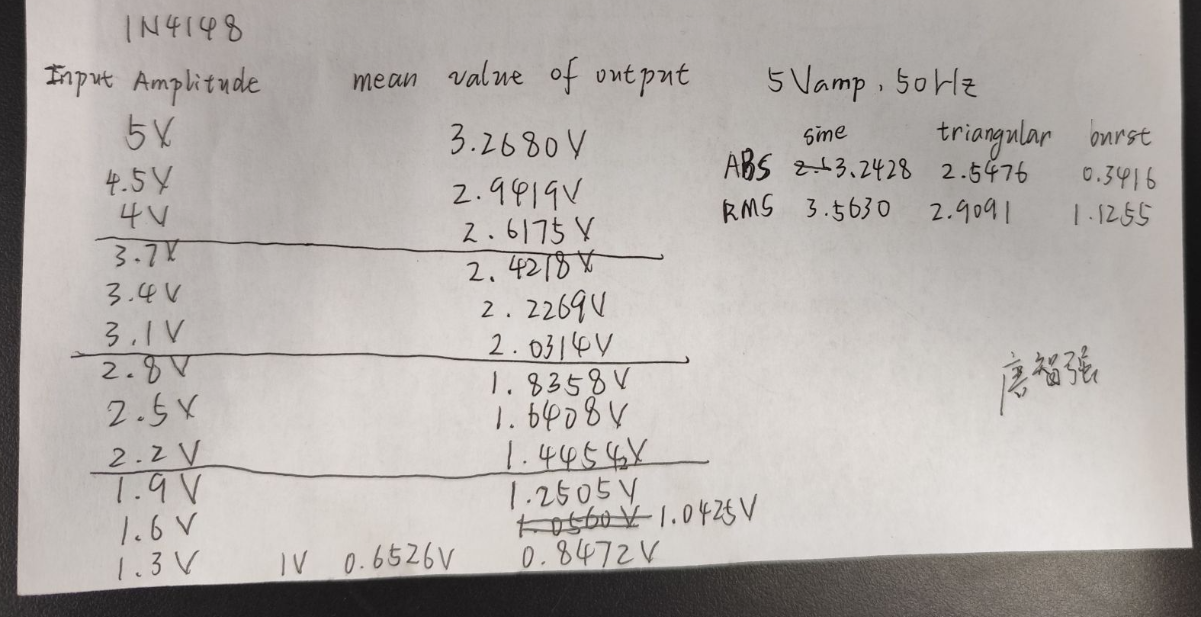
\includegraphics[width=\columnwidth]{LCE-05-精密整流/assets/appendix/image copy.png}
\end{figure}


% 附录
\section*{附录 C \hspace*{20pt} Matlab Codes}
\addcontentsline{toc}{section}{附录 C \hspace*{6pt} Matlab Codes} 
\thispagestyle{fancy} 
\lstinputlisting{D:/a_RemoteRepo/GH.MatlabCodes/本科课程代码/Linear Circuit Experiment/LCE_05.m}



\end{document}

% VScode 常用快捷键:

% F2:                       变量重命名
% Ctrl + Enter:             行中换行
% Alt + up/down:            上下移行
% 鼠标中键 + 移动:           快速多光标
% Shift + Alt + up/down:    上下复制
% Ctrl + left/right:        左右跳单词
% Ctrl + Backspace/Delete:  左右删单词    
% Shift + Delete:           删除此行
% Ctrl + J:                 打开 VScode 下栏(输出栏)
% Ctrl + B:                 打开 VScode 左栏(目录栏)
% Ctrl + `:                 打开 VScode 终端栏
% Ctrl + 0:                 定位文件
% Ctrl + Tab:               切换已打开的文件(切标签)
% Ctrl + Shift + P:         打开全局命令(设置)

% Latex 常用快捷键:

% Ctrl + Alt + J:           由代码定位到PDF


